%%%%%%%%%%%%%%%%%%%% book.tex %%%%%%%%%%%%%%%%%%%%%%%%%%%%%
%
% sample root file for the chapters of your "monograph"
%
% Use this file as a template for your own input.
%
%%%%%%%%%%%%%%%% Springer-Verlag %%%%%%%%%%%%%%%%%%%%%%%%%%


% RECOMMENDED %%%%%%%%%%%%%%%%%%%%%%%%%%%%%%%%%%%%%%%%%%%%%%%%%%%
\documentclass[pdftex,12pt, oneside]{article}

% choose options for [] as required from the list
% in the Reference Guide, Sect. 2.2
%\usepackage[paperwidth=8.5in, paperheight=13in]{geometry} % Folio
\usepackage[paperwidth=8.27in, paperheight=11.69in]{geometry} % A4

\usepackage{makeidx}         % allows index generation
\usepackage{graphicx}        % standard LaTeX graphics tool
                             % when including figure files
%\usepackage{multicol}        % used for the two-column index
\usepackage[bottom]{footmisc}% places footnotes at page bottom
\usepackage[bahasa]{babel}
\usepackage{enumerate}
\usepackage{paralist}
\usepackage{float}
\usepackage{gensymb}  
\usepackage{listings}
%\usepackage{siunitx}
% etc.
% see the list of further useful packages
% in the Reference Guide, Sects. 2.3, 3.1-3.3
\renewcommand{\baselinestretch}{1.5}

\newcommand{\HRule}{\rule{\linewidth}{0.5mm}}

%\makeindex             % used for the subject index
                       % please use the style svind.ist with
                       % your makeindex program


%%%%%%%%%%%%%%%%%%%%%%%%%%%%%%%%%%%%%%%%%%%%%%%%%%%%%%%%%%%%%%%%%%%%%

\begin{document}
\sloppy
%\author{Priyanto Tamami}
%\title{BUKU PETUNJUK OPERASIONAL SISTEM INFORMASI GEOGRAFIS UNTUK PBB-P2 DENGAN MAPINFO VERSI 8.0}
%\date{22 Desember 2015}
%\maketitle

%\input{./01.title.tex}
\begin{center}
{\large ANALISIS SISTEM OTENTIKASI PADA BADAN PENGELOLAAN PENDAPATAN, KEUANGAN DAN ASET DAERAH KABUPATEN BREBES}
\\[1cm]
15 Maret 2019\\
Priyanto Tamami, S.Kom.
\end{center}

%\frontmatter%%%%%%%%%%%%%%%%%%%%%%%%%%%%%%%%%%%%%%%%%%%%%%%%%%%%%%

%\include{dedic}
%\include{pref}

%\include{02.pengesahan} 

%\tableofcontents
%\listoffigures

%\mainmatter%%%%%%%%%%%%%%%%%%%%%%%%%%%%%%%%%%%%%%%%%%%%%%%%%%%%%%%
%\include{part}
%\include{chapter}
%\include{chapter}
%\appendix
%\include{appendix}

%\include{03.konsep-sig}
%\include{04.pengenalan-software}
%\include{05.koordinat}
%\include{06.registrasi-transformasi-koordinat} 
%\include{07.digitasi-on-screen} 
%\include{08.query} 

%\backmatter%%%%%%%%%%%%%%%%%%%%%%%%%%%%%%%%%%%%%%%%%%%%%%%%%%%%%%%
%\include{solutions}
%\include{referenc}
%\printindex

%%%%%%%%%%%%%%%%%%%%%%%%%%%%%%%%%%%%%%%%%%%%%%%%%%%%%%%%%%%%%%%%%%%%%%

\section{SASARAN DAN BATASAN SISTEM}

Sasaran dari sistem ini adalah mampu untuk melakukan otentikasi terhadap pengguna (\textit{resource owner}) yang melakukan akses ke \textit{resource server} melalui aplikasi klien (\textit{user agent}).

Batasan dari sistem ini yaitu hanya melingkupi proses otentikasi terhadap seluruh pengguna (\textit{resource owner}) yang telah terdaftar, kemudian memberikan hak kepada pengguna (\textit{resource owner}) yang karena kewenangannya ditunjuk sebagai administrator sistem, sehingga mampu untuk melakukan akses ke \textit{resource server} yang melayani pengaturan atau pengelolaan daftar pengguna (\textit{resource owner}) dan aplikasi klien (\textit{user agent}) di Badan Pengelolaan Pendapatan, Keuangan dan Aset Daerah Kabupaten Brebes.

\section{ARSITEKTUR SISTEM}


Seperti membangun sebuah gedung atau bangunan, agar bangunan dapat berdiri dengan kokoh dan memudahkan dalam pemeliharaan, maka diperlukan sebuah arsitektur, sedangkan pada pembuatan sistem aplikasi maka diperlukan sebuah arsitektur sistem aplikasi yang tujuannya pun agar kokoh dalam artian stabil dengan sedikit permasalahan yang muncul, dan memberikan kemudiahan pada saat pemeliharaan atau penambahan fitur pada sistem aplikasi yang sudah jadi.

Arsitektur sistem akan terbagi menjadi 3 (tiga) bagian, yaitu :

\begin{enumerate}[a.] 
	\item Bagian Basis Data
	\item Bagian Logika Aplikasi
	\item Bagian Tampilan Aplikasi
\end{enumerate}

\section{DESKRIPSI SUB SISTEM}

\subsection{Bagian Basis Data}

Pada bagian ini akan terdapat beberapa tabel yang digunakan untuk melakukan otentikasi pengguna (\textit{resource owner}) beserta hak aksesnya (\textit{role}), dan sebuah tabel yang digunakan untuk melakukan otorisasi bagi aplikasi klien (\textit{user agent}).

\subsection{Bagian Logika Aplikasi}

Pada bagian ini nantinya akan terdiri dari diagram struktur dan diagram perilaku dari aplikasi, bagaimana masing-masing komponen saling bertukar informasi, bagaimana alur data dari basis data ke bagian tampilan dan sebaliknya dimodelkan pada bagian ini.

Bagian ini bisa disebut inti dari aplikasi, karena bagian ini yang nantinya mengontrol transfer data antar komponen dan lapisan.

\subsection{Bagian Tampilan Aplikasi}

Istilah lainnya biasa dikenal dengan antar muka (\textit{user interface}) pengguna (\textit{resource owner}), bagian ini yang nantinya akan menjadi desain atau model dari tampilan yang berhadapan langsung dengan pengguna (\textit{resource owner}). Bagian ini yang nantinya mengumpulkan informasi untuk disampaikan kepada bagian logika aplikasi untuk diproses, bagian ini pula yang nantinya menampilkan informasi yang diproses oleh sistem untuk dapat dibaca dan dipahami oleh pengguna (\textit{resource owner}).

\section{PERTIMBANGAN KHUSUS KINERJA SISTEM}

Karena sistem datanya terpusat, yaitu tersimpan pada peladen (\textit{server}) basis data Postgresql, maka perawatan atau pemeliharaan mutlak harus dilakukan pada sisi peladen (\textit{server}) basis data yang diakibatkan dari peningkatan jumlah data transaksi perekaman yang selalu bertambah dan berubah dari sisi ukuran untuk setiap harinya.

Hal yang perlu dilakukan adalah pembersihan terhadap berkas \textit{log} (pencatatan), yaitu berkas yang digunakan oleh sistem basis data PostgresSQL untuk mencatatkan kegiatan atau aktivitas yang telah dilakukannya selama beroperasi melayani permintaan data. Pembersihan ini dilakukan secara periodik karena transaksi perubahan yang terjadi sifatnya insidental, sehingga kegiatan ini dapat dilakukan dalam rentang bulanan.

Selain peladen (\textit{server}) sistem basis data, peladen (\textit{server}) aplikasi \textit{web} pun perlu mendapatkan perhatian pada sisi perawatan atau pemeliharaan, dimana peladen (\textit{server}) aplikasi \textit{web} pun memiliki berkas \textit{log} tersendiri yang perlu dibersihkan secara rutin karena menyimpan transaksi antara komputer klien dan peladen (\textit{server}).

Hal lain yang perlu dilakukan sebagai langkah pengamanan data yaitu dilakukannya duplikasi data (\textit{backup data}) sehingga apabila terjadi hal-hal yang tidak diinginkan, data dapat langsung dikembalikan atau dipulihkan (\textit{recovery}). Ini pun sebaiknya dilakukan secara rutin, sebaiknya dalam periode harian.

\section{HASIL PEMODELAN}

Hasil pemodelan untuk sistem otentikasi ini nantinya akan dibagi menjadi beberapa diagram dasar pada beberapa bagian dari arsitektur sistem, berikut rincian mengenai hasil pemodelan tersebut :

\subsection{Bagian Basis Data}

Struktur basis data yang dibangun untuk kebutuhan sistem otentikasi pada Badan Pengelolaan Pendapatan, Keuangan dan Aset Daerah Kabupaten Brebes adalah seperti pada gambar \ref{fig:db-dia} berikut ini :

\begin{figure}[H]
	\centering
	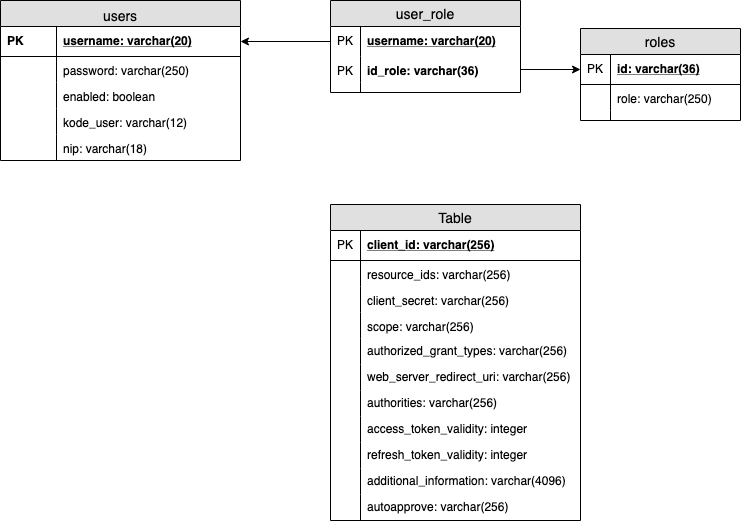
\includegraphics[width=1\textwidth]{./resources/db-diagram}
	\caption{Diagram Tabel Yang Digunakan}
	\label{fig:db-dia}
\end{figure}


\subsection{Bagian Logika Aplikasi}

Ada beberapa pemodelan logika aplikasi di dunia teknologi informasi, jika pengembangan dilakukan dengan bahasa pemrograman terstruktur, maka akan menggunakan \textit{flowchart} atau diagram alir sebagai alat untuk pemodelan, karena yang akan digunakan sekarang adalah bahasa pemrograman Kotlin yang menggunakan metodologi orientasi objek, maka digunakan \textit{Unified Modeling Language} (UML) yang akan menggambarkan struktur sistem dari awal sampai akhir. Berikut adalah pemodelan atau diagram yang menggambarkan bagian sistem otentikasi pada Badan Pengelolaan Pendapatan, Keuangan dan Aset Daerah Kabupaten Brebes bekerja.

\subsubsection{Diagram \textit{Use Case}}

Diagram \textit{use-case} dari keseluruhan sistem yang akan dibangun adalah seperti gambar \ref{fig:use-case} ini :

\begin{figure}[H]	
	\centering
	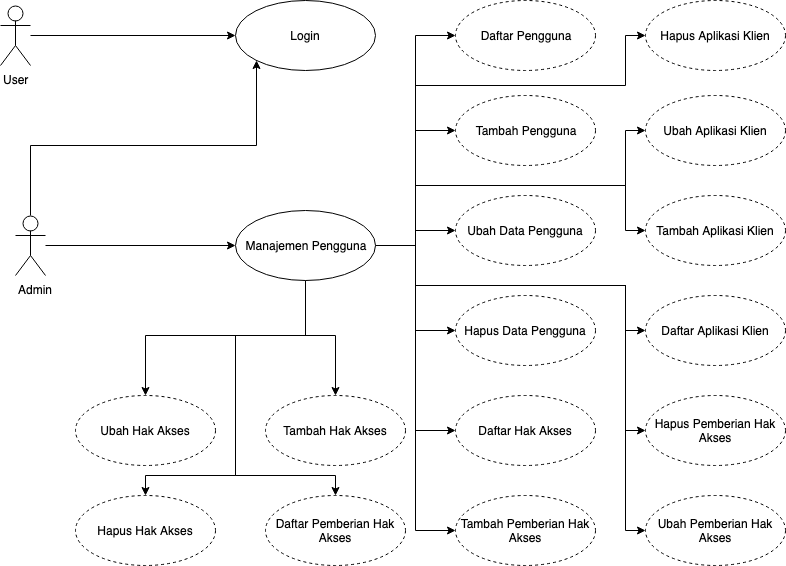
\includegraphics[width=1\textwidth]{resources/use-case-diag}
	\caption{Diagram \textit{Use-Case}}
	\label{fig:use-case}
\end{figure}

Sistem otentikasi hanya akan menampilkan halaman \textit{login} saja bagi pengguna selain administrator, namun yang memiliki kewenangan sebagai administrator dapat melakukan akses ke manajemen atau pengelolaan daftar pengguna setelah melakukan \textit{login} pada aplikasi klien (\textit{user agent})

\subsubsection{Diagram \textit{Class}}

Diagram \textit{class} pada sistem otentikasi ini akan terbagi menjadi 3 (tiga) bagian, yaitu pada \textit{OAuth Server}, \textit{Resource Server}, dan aplikasi klien (\textit{user agent}).

Diagram \textit{class} untuk \textit{OAuth Server} sendiri akan menjadi beberapa bagian yang dipisahkan dengan penamaan paketnya, berikut adalah daftar paket yang membentuk sebuah \textit{OAuth Server} : 

\begin{enumerate}

	\item Paket yang pertama yaitu \texttt{lab.aikibo.oauthbppkad.config} yang terlihat seperti pada gambar \ref{fig:class-dia-oauth} berikut ini :

\begin{figure}[H]
	\centering
	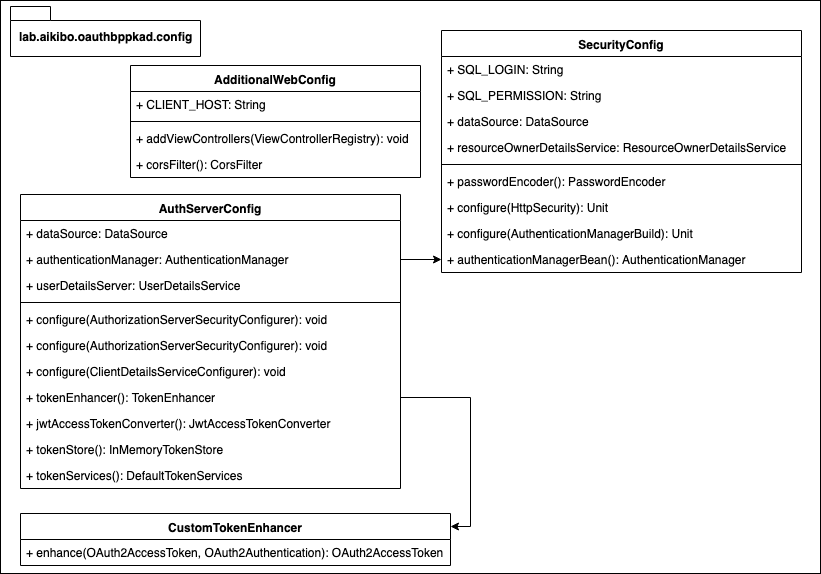
\includegraphics[width=1\textwidth]{./resources/class-dia-oauth}
	\caption{Diagram \textit{Class} OAuth Bagian 1}
	\label{fig:class-dia-oauth}
\end{figure}

	Paket ini berhubungan dengan konfigurasi yang terjadi untuk memberikan layanan \textit{service} \textit{OAuth} yang ditawarkan.
	
	\item Paket berikutnya adalah \texttt{lab.aikibo.oauthbppkad.entity.id} yang berisi kelas-kelas pembentuk \textit{primary key} dari tabel yang memiliki \textit{composite key} atau bentuk \textit{primary key} yang terdiri dari beberapa \textit{field} atau kolom. Berikut adalah diagram \textit{class} pembentuknya :

\begin{figure}[H]
	\centering
	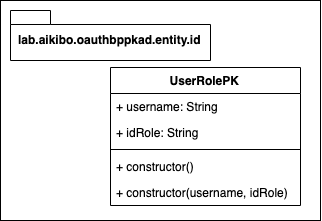
\includegraphics[width=0.5\textwidth]{./resources/class-dia-oauth-1}
	\caption{Diagram \textit{Class} OAuth Bagian 2}
	\label{fig:class-dia-oauth-1}
\end{figure}

	\item Paket berikutnya adalah \texttt{lab.aikibo.oauthbppkad.entity} yang terdiri dari beberapa kelas entitas yang digunakan untuk memetakan struktur tabel pada sistem database ke dalam objek Kotlin. Berikut adalah diagram \textit{class} dari paket ini :

\begin{figure}[H]
	\centering
	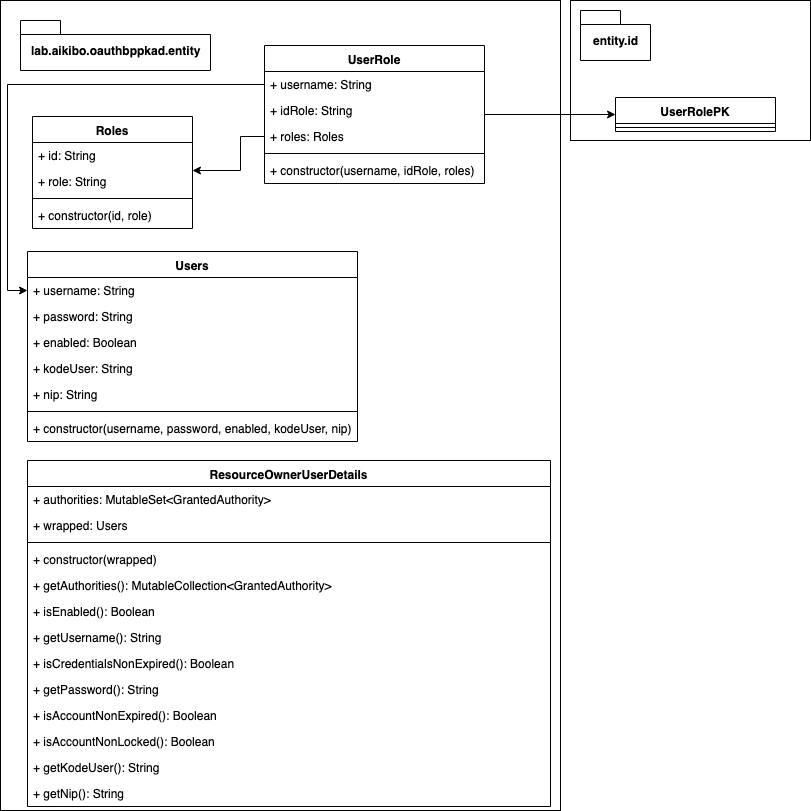
\includegraphics[width=1\textwidth]{./resources/class-dia-oauth-2}
	\caption{Diagram \textit{Class} OAuth Bagian 3}
	\label{fig:class-dia-oauth-2}
\end{figure}

	\item Paket berikutnya adalah \texttt{lab.aikibo.oauthbppkad.repo} yang berisi dari deklarasi \textit{interface} dimana fungsinya adalah untuk melakukan operasi manipulasi data pada sistem basis data. Daftar \textit{interface} dari paket ini adalah seperti berikut :

\begin{figure}[H]
	\centering
	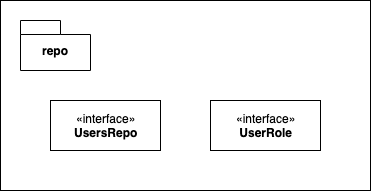
\includegraphics[width=0.5\textwidth]{./resources/class-dia-oauth-3}
	\caption{Diagram \textit{Class} OAuth Bagian 4}
	\label{fig:class-dia-oauth-3}
\end{figure}

	\item Paket berikutnya adalah \texttt{lab.aikibo.oauthbppkad.services} yang berisi kelas-kelas pengolah data baik yang akan disimpan melalui \textit{interface-interface} di paket \texttt{repo}, atau yang datang dari paket \texttt{repo} untuk kemudian dikirimkan ke luar. Berikut adalah kelas pembentuk dari paket ini :

\begin{figure}[H]
	\centering
	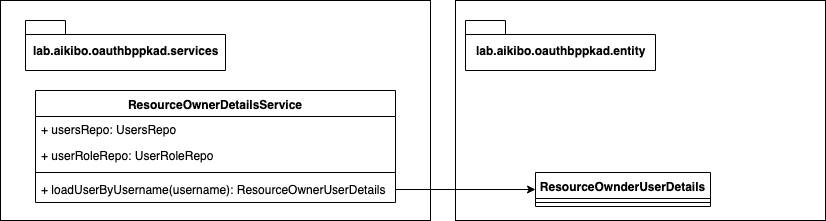
\includegraphics[width=1\textwidth]{./resources/class-dia-oauth-4}
	\caption{Diagram \textit{Class} OAuth Bagian 5}
	\label{fig:class-dia-oauth-4}
\end{figure}

	\item Paket berikutnya adalah \texttt{lab.aikibo.oauthbppkad} yang berisi sebuah kelas yang nantinya akan dieksekusi pertama kali saat layanan dari \textit{OAuth Server} berjalan. Berikut adalah diagram \textit{class} dari paket ini :

\begin{figure}[H]
	\centering
	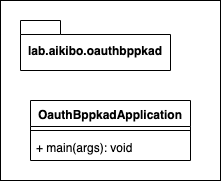
\includegraphics[width=0.4\textwidth]{./resources/class-dia-oauth-5}
	\caption{Diagram \textit{Class} OAuth Bagian 6}
	\label{fig:class-dia-oauth-5}
\end{figure}

\end{enumerate}

Diagram \textit{class} untuk \textit{Resource Server} pun akan terdiri dari beberapa paket untuk memperjelas bagan dari diagram \textit{class} yang terbentuk, berikut adalah daftarnya :

\begin{enumerate}

	\item Paket \texttt{lab.aikibo.userservice} akan terdiri dari sebuah kelas saja, dimana kelas ini akan dijalankan pertama kali saat layanan dari \textit{Resource Server} memulai aktivitasnya. Diagram \textit{class} dari paket ini adalah seperti berikut :
	
	\begin{figure}[H]
		\centering
		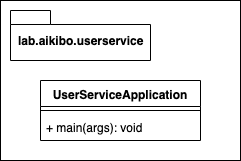
\includegraphics[width=0.3\textwidth]{./resources/class-dia-resource-1}
		\caption{Diagram \textit{Class Resource Server} Bagian 1}
		\label{fig:class-dia-resource-1}
	\end{figure}
	
	\item Paket \texttt{lab.aikibo.userservice.config} akan terdiri dari beberapa kelas untuk melakukan konfigurasi \textit{Resource Server}. Diagram \textit{class} dari paket ini adalah seperti berikut :
	
	\begin{figure}[H]
		\centering
		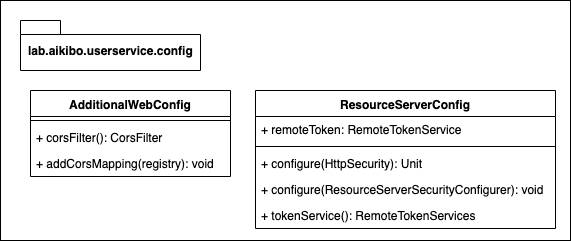
\includegraphics[width=0.8\textwidth]{./resources/class-dia-resource-2}
		\caption{Diagram \textit{Class Resource Server} Bagian 2}
		\label{fig:class-dia-resource-2}
	\end{figure}
	
	\item Paket \texttt{lab.aikibo.userservice.controller} akan terdiri dari beberapa kelas yang mendefinisikan URI (\textit{Uniform Resource Identifier}) dari layanan yang diberikan oleh \textit{Resource Server}. Berikut adalah diagram \textit{class} untuk paket ini :
	
	\begin{figure}[H]
		\centering
		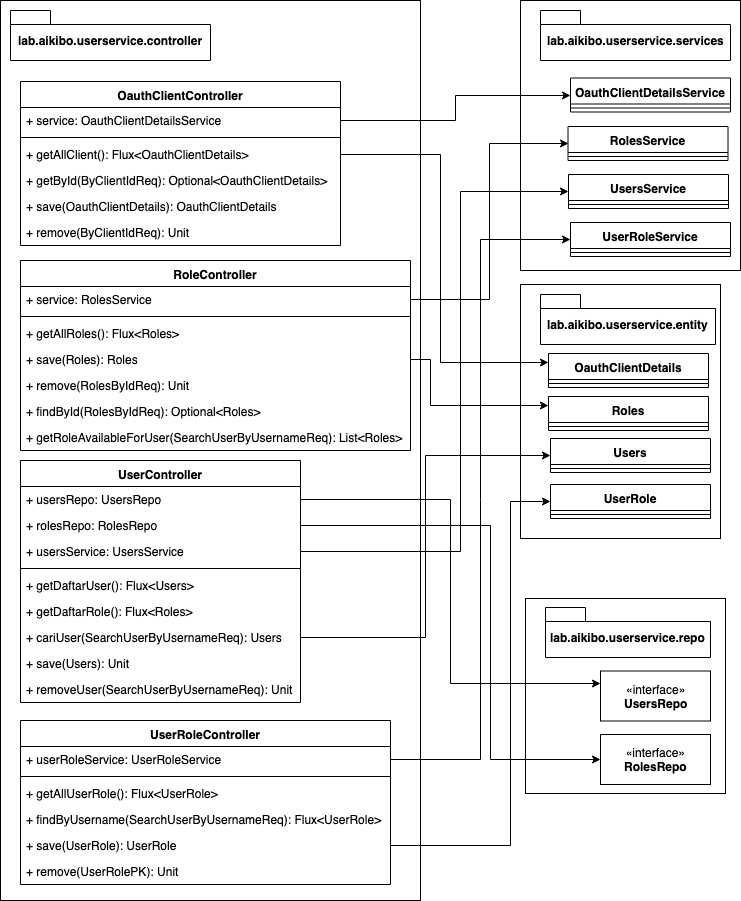
\includegraphics[width=1\textwidth]{./resources/class-dia-resource-3}
		\caption{Diagram \textit{Class Resource Server} Bagian 3}
		\label{fig:class-dia-resource-3}
	\end{figure}
	
	\item Paket \texttt{lab.aikibo.userservice.entity.id} akan terdiri dari kelas-kelas pembentuk \textit{primary key} bagi tabel yang memiliki \textit{primary key} berupa \textit{composite key} atau lebih dari 1 (satu) \textit{field} atau kolom. Diagram kelas dari paket ini adalah seperti berikut :
	
	\begin{figure}[H]
		\centering
		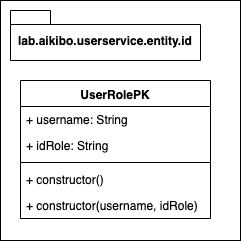
\includegraphics[width=0.3\textwidth]{./resources/class-dia-resource-4}
		\caption{Diagram \textit{Class Resource Server} Bagian 4}
		\label{fig:class-dia-resource-4}
	\end{figure}
	
	\item Paket \texttt{lab.aikibo.userservice.entity} akan terdiri dari kelas-kelas yang digunakan untuk memetakan tabel ke dalam objek Kotlin, jadi tiap tabel yang terdapat pada sistem basis data, akan memiliki pasangan masing-masing di objek Kotlin. Gambar diagram \textit{class} dari paket ini adalah seperti berikut :
	
	\begin{figure}[H]
		\centering
		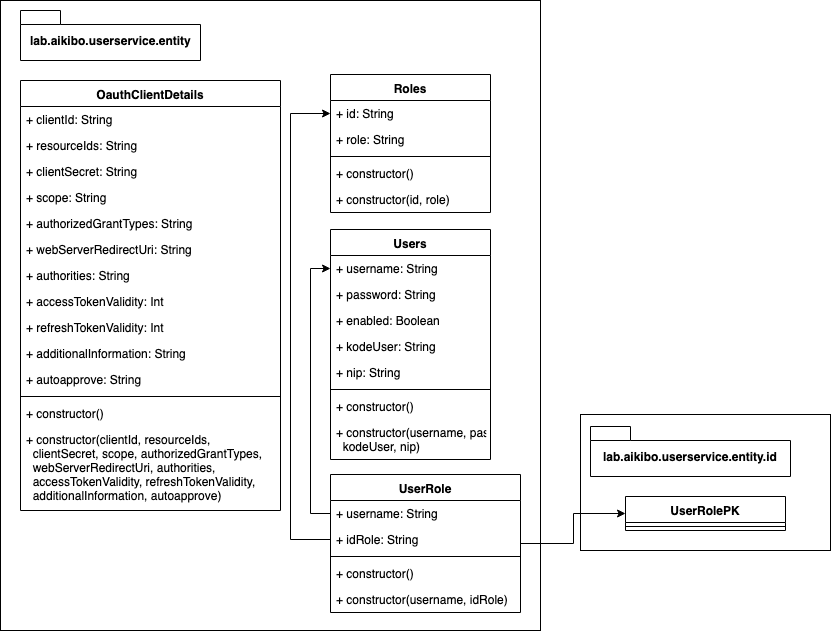
\includegraphics[width=1\textwidth]{./resources/class-dia-resource-5}
		\caption{Diagram \textit{Class Resource Server} Bagian 5}
		\label{fig:class-dia-resource-5}
	\end{figure}
	
	\item Paket \texttt{lab.aikibo.userservice.model} akan terdiri dari kelas-kelas yang digunakan untuk pemetaan objek JSON yang datang dari \textit{request} aplikasi klien (\textit{user agent}). Terkadang kelas-kelas yang di dalam paket ini pun difungsikan untuk membentuk objek JSON sebagai \textit{response} atau \textit{request} yang terjadi dari aplikasi klien (\textit{user agent}). Diagram \textit{class} untuk paket ini adalah seperti berikut :
	
	\begin{figure}[H]
		\centering
		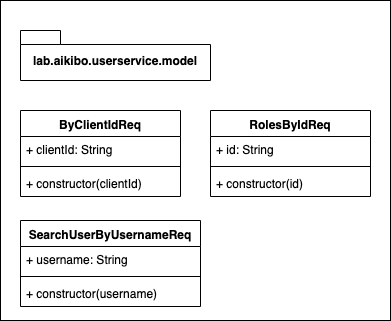
\includegraphics[width=0.5\textwidth]{./resources/class-dia-resource-6}
		\caption{Diagram \textit{Class Resource Server} Bagian 6}
		\label{fig:class-dia-resource-6}
	\end{figure} 
	
	\item Paket \texttt{lab.aikibo.userservice.repo} akan terdiri dari beberapa \textit{interface} yang fungsinya adalah untuk melakukan manipulasi data pada sistem basis data. Diagram \textit{class} dari paket ini adalah seperti gambar berikut :
	
	\begin{figure}[H]
		\centering
		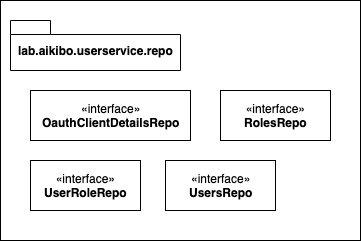
\includegraphics[width=0.5\textwidth]{./resources/class-dia-resource-7}
		\caption{Diagram \textit{Class Resource Server} Bagian 7}
		\label{fig:class-dia-resource-7}
	\end{figure}
	
	\item Paket \texttt{lab.aikibo.userservice.services} akan terdiri dari beberapa kelas yang fungsinya untuk melakukan penyesuaian parameter pada saat akan melakukan manipulasi di sistem basis data melalui \textit{interface} pada paket \texttt{repo}, atau pada saat melakukan pengambilan nilai dari sistem basis data. Diagram \textit{class} untuk paket ini adalah seperti berikut :
	
	\begin{figure}[H]
		\centering
		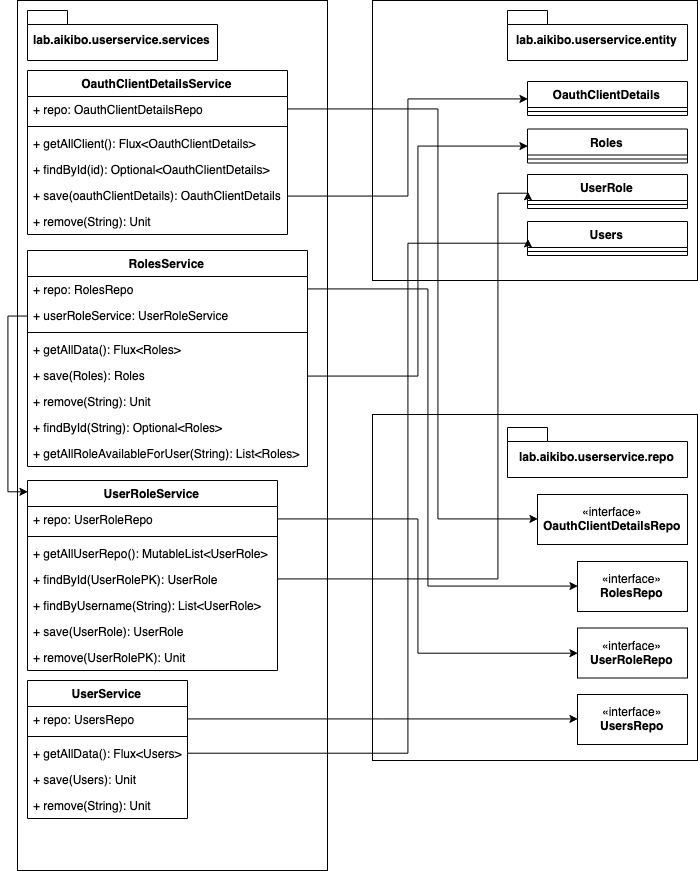
\includegraphics[width=1\textwidth]{./resources/class-dia-resource-8}
		\caption{Diagram \textit{Class Resource Server} Bagian 8}
		\label{fig:class-dia-resource-8}
	\end{figure}

\end{enumerate}

Sekarang ke bagian \textit{front-end} yang akan dibangun dengan Angular . Karena menganut konsep \textit{Object Oriented} juga, sehingga kita dapat melakukan pemodelan dengan UML, termasuk diagram \textit{class} yang akan dibangun. 

Untuk membentuk rangka dari aplikasi klien (\textit{user agent}), beberapa kelas yang dibutuhkan akan terdapat pada diagram \textit{class} berikut :

\begin{figure}[H]
	\centering
	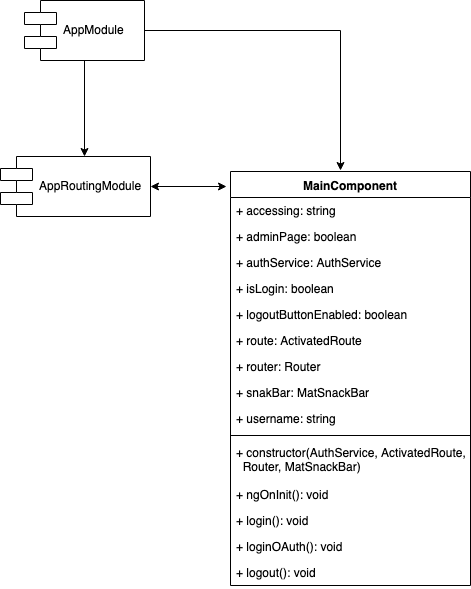
\includegraphics[width=0.8\textwidth]{./resources/class-dia-fe-1}
	\caption{Diagram \textit{Class} Aplikasi Klien Bagian 1}
	\label{fig:class-dia-fe-1}
\end{figure}

Untuk aplikasi klien (\textit{user agent}) pengelolaan daftar pengguna akan terdiri dari beberapa kelas pembentuk seperti diagram \textit{class} berikut :

\begin{figure}[H]
	\centering
	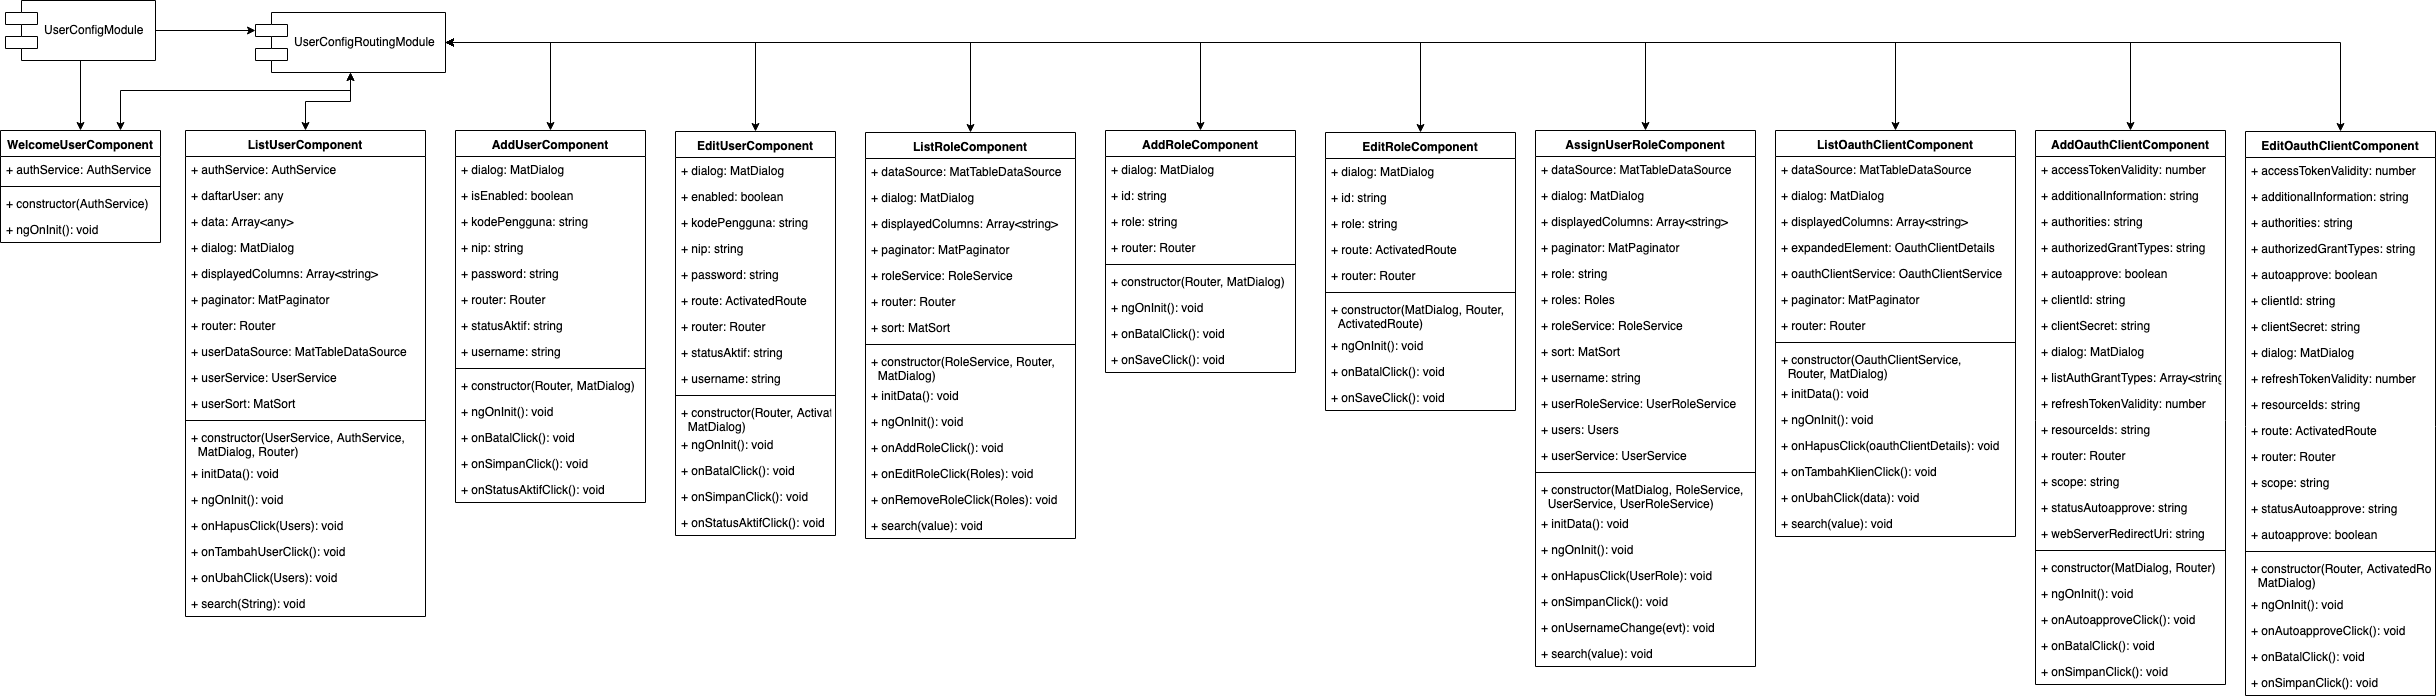
\includegraphics[width=1\textwidth]{./resources/class-dia-fe-2}
	\caption{Diagram \textit{Class} Aplikasi Klien Bagian 2}
	\label{fig:class-dia-fe-2}
\end{figure}

Adapun kelas-kelas pendukung yang digunakan untuk melakukan akses ke \textit{resource server} dilakukan oleh beberapa \textit{services}, berikut adalah diagram \textit{class} dari kelas-kelas pendukung tersebut :

\begin{figure}[H]
	\centering
	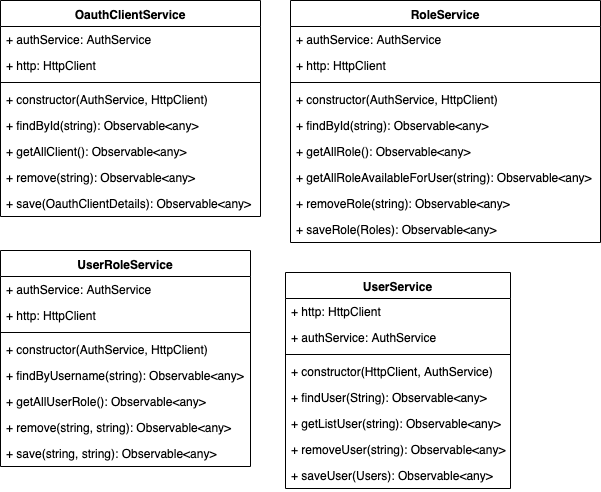
\includegraphics[width=1\textwidth]{./resources/class-dia-services}
	\caption{Diagram \textit{Class Services}}
	\label{fig:class-dia-services}
\end{figure}

Berikutnya adalah kelas-kelas yang membentuk jendela dialog yang digunakan untuk menampilkan informasi terbatas bagi pengguna aplikasi, diagram \textit{class} dari jendela dialog ini adalah seperti berikut :

\begin{figure}[H]
	\centering
	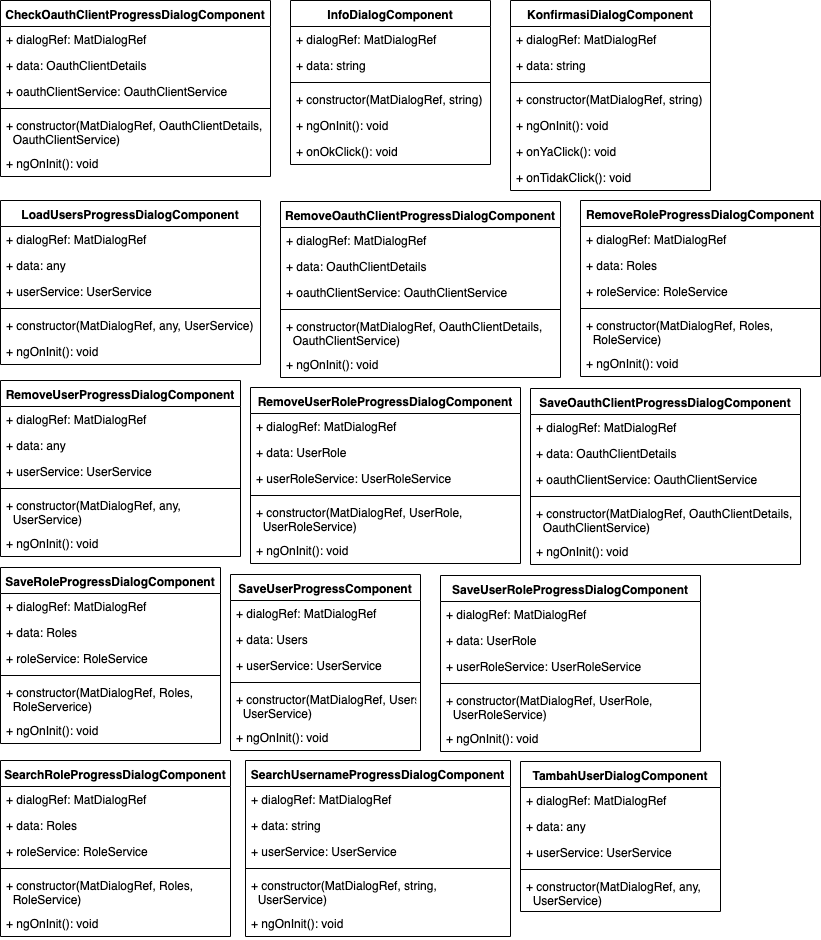
\includegraphics[width=1\textwidth]{./resources/class-dia-dialog}
	\caption{Diagram \textit{Class} untuk \textit{Dialog}}
	\label{fig:class-dia-dialog}
\end{figure}

\subsubsection{Diagram \textit{Package}}

Diagram ini akan menunjukan struktur desain sistem pada level \textit{package}. Diagram \textit{package} untuk \textit{oauth server} adalah seperti pada gambar \ref{fig:package-dia-oauth-server} berikut ini :

\begin{figure}[H]
	\centering
	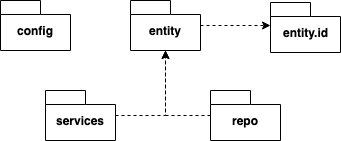
\includegraphics[width=0.5\textwidth]{./resources/package-dia-oauth-server}
	\caption{Diagram \textit{Package} pada \textit{OAuth Server}}
	\label{fig:package-dia-oauth-server}
\end{figure}

Berikut penjelasan dari tiap \textit{package} :

\begin{enumerate}

	\item \textit{Package} \texttt{config} berfungsi untuk melakukan konfigurasi terhadap \textit{Oauth Server} yang akan berjalan, yang tidak berkait dengan beberapa \textit{package} lainnya.
	
	\item \textit{Package} \texttt{entity.id} ini sebagai wadah dari kelas-kelas pembentuk \textit{primary key} yang digunakan oleh kelas-kelas yang terdapat dalam \textit{package} \texttt{entity}.
	
	\item \textit{Package} \texttt{entity} berisi kelas-kelas yang digunakan untuk memetakan tabel dari sistem basis data.
	
	\item \textit{Package} \texttt{repo} berisi \textit{interface} untuk melakukan operasi data ke sistem basis data.
	
	\item \textit{Package} \texttt{services} berisi kelas-kelas yang melakukan pengolahan data sebelum dilakukan proses simpan data ke sistem basis data atau setelah melakukan pengambilan data dari sistem basis data.
	
\end{enumerate}

Diagram \textit{package} untuk \textit{resource server} adalah seperti pada gambar berikut :

\begin{figure}[H]
	\centering
	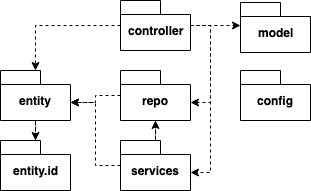
\includegraphics[width=0.5\textwidth]{./resources/package-dia-resource-server}
	\caption{Diagram \textit{Package} pada \textit{Resource Server}}
	\label{fig:package-dia-resource-server}
\end{figure}

Penjelasan dari paket-paket tersebut adalah seperti berikut ini :

\begin{enumerate}
	\item \textit{Package} \texttt{entity} adalah tempat bagi kelas-kelas yang digunakan untuk memetakan tabel-tabel yang terdapat dalam basis data.
	
	\item \textit{Package} \texttt{entity.id} adalah tempat untuk kelas-kelas yang menjadi definisi \textit{primary key} bagi kelas-kelas entitas yang terdapat pada \textit{package} \texttt{entity}.
	
	\item \textit{Package} \texttt{controller} adalah tempat bagi kelas-kelas yang mendefinisikan URI (\textit{Uniform Resource Identifier}) dari layanan-layanan yang diberikan oleh \textit{Resource Server}.
	
	\item \textit{Package} \texttt{repo} adalah tempat bagi \textit{interface-interface} yang digunakan untuk melakukan akses atau operasi data pada sistem basis data.
	
	\item \textit{Package} \texttt{services} adalah tempat bagi kelas-kelas yang melakukan adaptasi data yang akan disimpan pada sistem basis data atau akan ditampilkan dari sistem basis data.
	
	\item \textit{Package} \texttt{model} adalah tempat bagi kelas-kelas yang digunakan sebagai \textit{model} untuk melakukan \textit{respon} atau menerima \textit{request} dari aplikasi klien (\textit{user agent}). Nantinya kelas-kelas di dalam \textit{package} ini akan secara otomatis dikonversi ke dalam JSON atau sebaliknya, dari format JSON akan bentuk ke dalam objek-objek dari kelas-kelas dalam \textit{package} ini.
	
	\item \textit{Package} \texttt{config} adalah tempat bagi kelas-kelas yang melakukan konfigurasi \textit{framework} dari \textit{Resource Server}.
	
\end{enumerate}

Untuk bagian \textit{User Interface} atau dalam hal ini adalah aplikasi klien (\textit{user agent}), karena tidak berbentuk paket seperti halnya pada Kotlin, untuk memudahkan akan dianalogikan sebuah paket adalah sebuah kandar / direktori dari tiap kelas yang terbentuk. Diagram \textit{package} dari bagian \textit{front-end} adalah seperti berikut :

\begin{figure}[H]
	\centering
	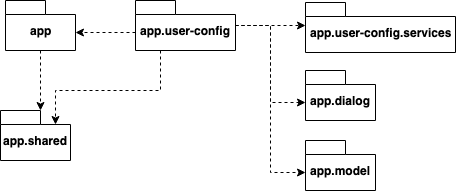
\includegraphics[width=0.7\textwidth]{./resources/package-dia-fe}
	\caption{\textit{Package} Diagram dari \textit{Front-End}}
	\label{fig:package-dia-fe}
\end{figure}

Penjelasan dari tiap \textit{package} di atas adalah seperti berikut :

\begin{enumerate}
	\item \textit{Package} \texttt{app} adalah paket utama dari \textit{project} yang dibangun, nantinya \textit{routing} akan diatur dalam \textit{package} ini yang akan bergantung pada otorisasi dari \textit{package} \texttt{app.shared}.
	
	\item \textit{Package} \texttt{app.shared} adalah paket yang berisi kelas-kelas pendukung yang nantinya akan digunakan dari seluruh \textit{package} untuk menentukan otentikasi yang didapat, dan alamat dari \textit{service-service} yang dapat diakses.
	
	\item \textit{Package} \texttt{app.user-config} akan berisi kelas-kelas pembentuk tampilan tatap muka (\textit{user interface}) dari aplikasi manajemen pengguna.
	
	\item \textit{Package} \texttt{app.user-config.services} akan berisi kelas-kelas yang berfungsi untuk menyediakan akses atau operasi data dari dan ke \textit{resource server}.
	
	\item \textit{Package} \texttt{app.dialog} akan berisi berbagai macam kelas yang berbentuk tampilan \textit{dialog} untuk menampilkan berbagai macam informasi seperti proses simpan data, proses unduh data, konfirmasi aksi, informasi kesalahan, dan sebagainya.
	
	\item \textit{Package} \texttt{app.model} akan berisi dari objek-objek yang digunakan untuk menerima \textit{response} dari atau mengirimkan \textit{request} ke \textit{resource server} dalam format JSON.
\end{enumerate}

\subsubsection{Diagram \textit{Component}}

% liat disini -> http://www.uml-diagrams.org/communication-diagrams-examples.html

Diagram ini memberikan gambaran hubungan antar komponen, komponen mana yang membutuhkan data dan komponen mana yang memberikan data akan terlihat jelas pada diagram komponen ini. Berikut adalah diagram \textit{component} yang terbagi menjadi beberapa bagian berdasarkan fungsinya :

\begin{enumerate}
	\item Diagram \textit{Component} pada \textit{Oauth Server} akan terlihat seperti pada gambar berikut :
	
	\begin{figure}[H]
		\centering
		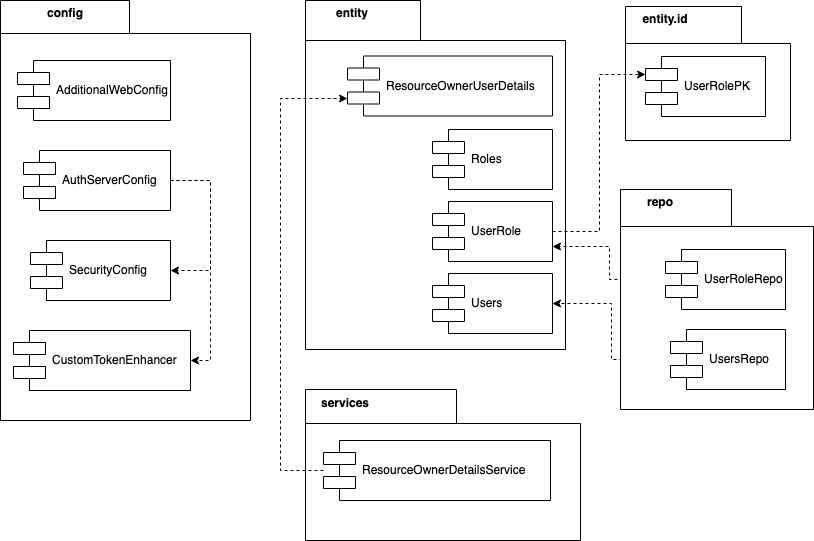
\includegraphics[width=1\textwidth]{./resources/comp-dia-oauth}
		\caption{Diagram \textit{Component} Untuk \textit{Oauth Server}}
		\label{fig:comp-dia-oauth}
	\end{figure}
	
	\item Diagram \textit{Component} pada \textit{Resource Server} akan terlihat seperti pada gambar berikut :
	
	\begin{figure}[H]
		\centering
		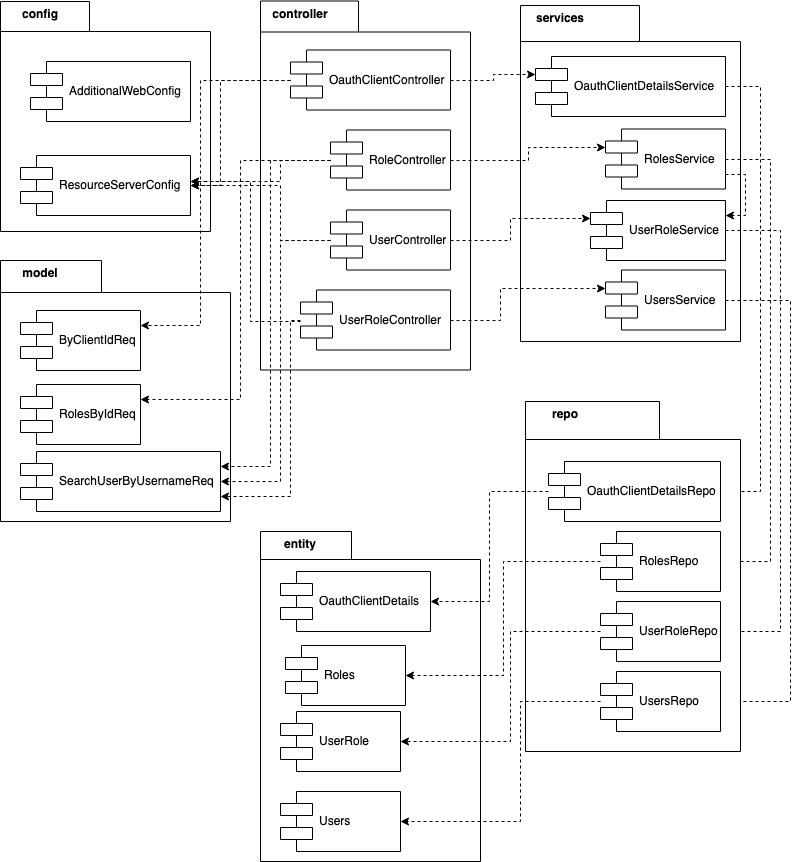
\includegraphics[width=1\textwidth]{./resources/comp-dia-resource}
		\caption{Diagram \textit{Component} untuk \textit{Resource Server}}
		\label{fig:comp-dia-resource}
	\end{figure}
	
	\item Diagram \textit{Component} pada Aplikasi Klien (\textit{User Agent}) adalah seperti terlihat pada gambar berikut :
	
	\begin{figure}[H]
		\centering
		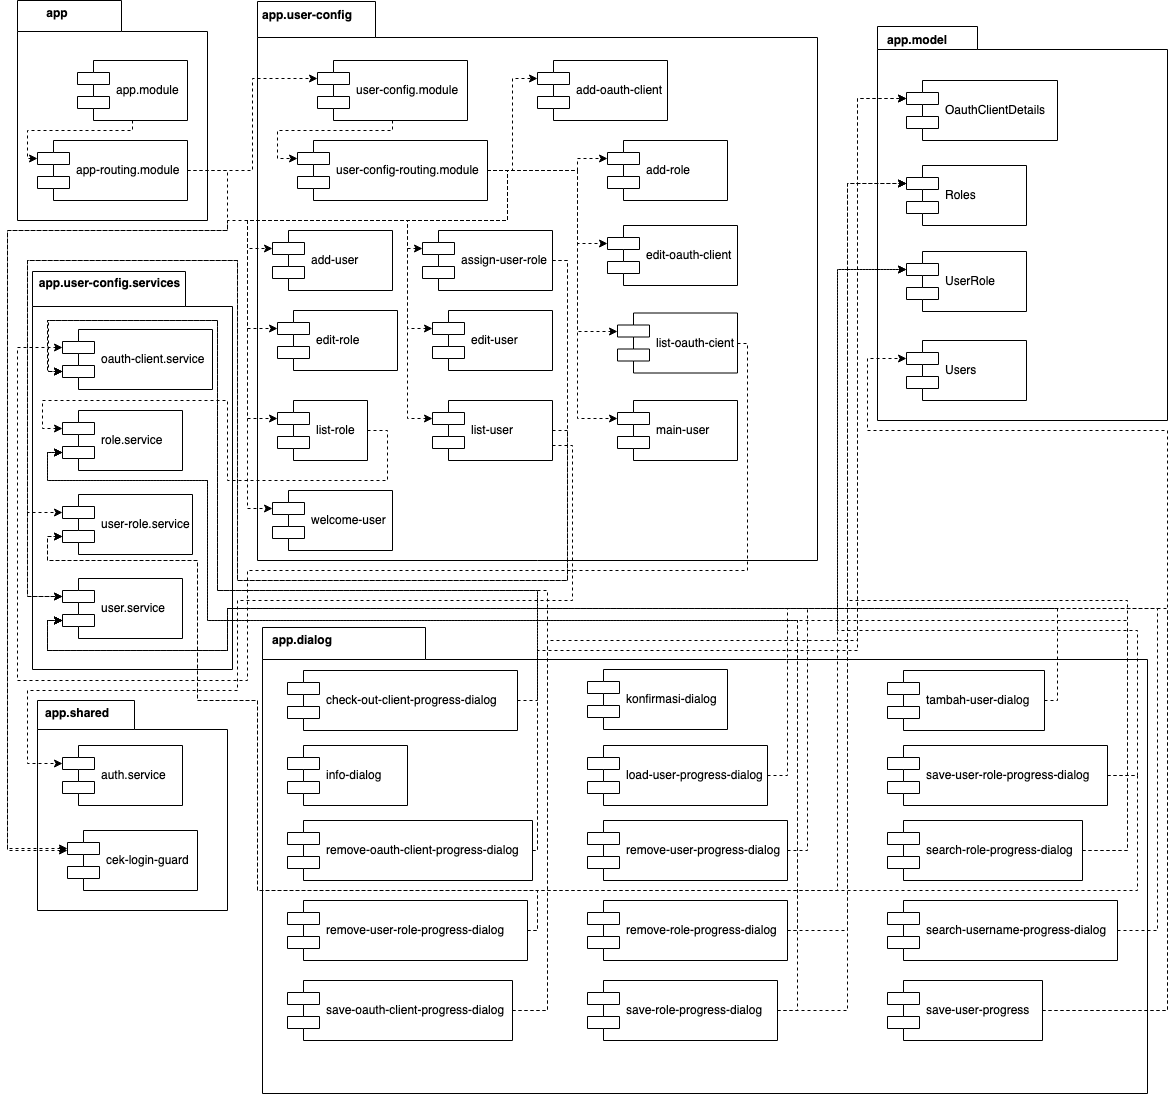
\includegraphics[width=1\textwidth]{./resources/comp-dia-fe}
		\caption{Diagram \textit{Component} Untuk Aplikasi Klien (\textit{User Agent})}
		\label{fig:comp-dia-fe}
	\end{figure}
\end{enumerate}

Diagram ini berisi komponen-komponen yang membangun sistem ini menjadi utuh, diagram ini digunakan untuk menjabarkan artifak sistem secara fisik, dimana berkas harus ditempatkan, apa saja nama paket / kandarnya, dan hubungan antar \textit{class} atau berkas, kemana data atau proses berikutnya akan berjalan.


\subsubsection{Diagram \textit{Deployment}}

Diagram ini menunjukkan arsitektur dari sistem pada saat didistribusikan dari mesin tempat untuk mengembangan dan uji coba, ke mesin produksi tempat aplikasi siap untuk melayani pengguna aslinya.

Diagram \textit{deployment} terlihat seperti pada gambar berikut :

\begin{figure}[H]
	\centering
	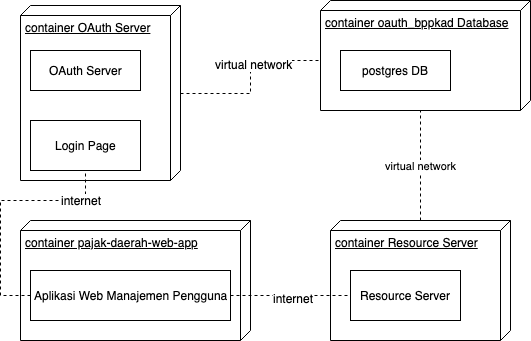
\includegraphics[width=1\textwidth]{./resources/deploy-dia}
	\caption{Diagram \textit{Deployment}}
	\label{fig:deploy-dia}
\end{figure}

Pada diagram tersebut ditunjukkan bahwa akan ada 4 (empat) docker \textit{container} yang masing-masing \textit{container} memiliki layanannya sendiri, pengguna nantinya hanya akan terhubung melalui \textit{container} \textbf{pajak-daerah-web-app} karena ini adalah tatap muka (\textit{user interface}) yang dapat diakses oleh pengguna, kemudian saat pengguna akan melakukan akses terhadap data sensitif, pengguna akan diarahkan (\textit{redirect}) ke halaman \textit{login} untuk melakukan otentikasi, setelah itu akan diarahkan kembali ke Aplikasi Web Manajemen Pengguna, semua aktitifas pengguna akan terjadi pada layanan ini.

Simpanan data / basis data akan terhubung dengan \textit{OAuth Server} dan \textit{Resource Server} melalui jaringan virtual yang digunakan sebagai tempat simpanan data dari daftar pengguna (\textit{resource owner}) dan daftar aplikasi klien (\textit{user agent}).

Komunikasi antara Aplikasi Web Manajemen Pengguna dengan \textit{Resource Server} akan sering terjadi setiap pengguna melakukan operasi data. Komunikasi akan terjalin menggunakan arsitektur REST dengan bentuk JSON sebagai format pertukaran datanya.

\subsubsection{Diagram \textit{Communication}}

Diagram ini menggambarkan interaksi antar objek yang disertai urutan komunikasi dalam bentuk bagan yang bebas. Diagram ini akan terbagi menjadi beberapa bagian berdasarkan fitur yang diberikan oleh sistem otentikasi, berikut adalah daftar diagram yang terbentuk :

\begin{itemize}
	\item Fitur \textit{Login}
	
	Diagram \textit{communication} untuk fitur ini akan menjelaskan proses yang terjadi pada saat pengguna (\textit{resource owner}) melakukan otentikasi aplikasi, prosesnya akan terlihat seperti gambar diagram \textit{communication} berikut :
	
	\begin{figure}[H]
		\centering
		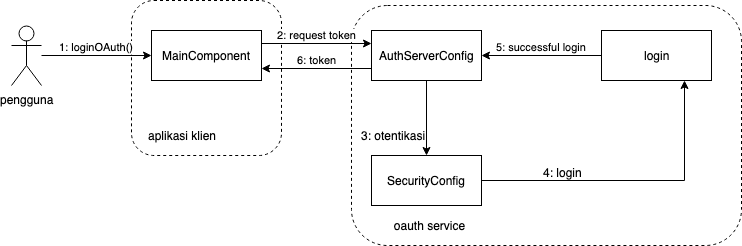
\includegraphics[width=1\textwidth]{./resources/comm-dia-login}
		\caption{Diagram \textit{Communication} Untuk Fitur \textit{Login}}
		\label{fig:comm-dia-login}
	\end{figure}
	
	Skenario proses yang terjadi adalah seperti berikut :
	
	\begin{enumerate}
		\item Pengguna mulai melakukan akses ke aplikasi klien (\textit{user agent})
		\item Aplikasi klien (\textit{user agent}) melakukan \textit{request} token ke \textit{OAuth Server}.
		\item \textit{OAuth Server} melakukan otentikasi dan verifikasi \textit{request} terhadap Pengguna (\textit{resource owner}) dan aplikasi klien (\textit{user agent})
		\item \textit{OAuth Server} akan mengarahkan pengguna ke halaman \textit{login}.
		\item Setelah proses di halaman \textit{login} berhasil diverifikasi, proses selanjutnya kembali ke kelas \texttt{AuthServerConfig} untuk membuat sebuah token berdasarkan pengguna yang telah melakukan \textit{login}.
		\item \textit{OAuth Server} mengirimkan token JWT ke aplikasi klien (\textit{user agent})
	\end{enumerate}
	
	\item Fitur Tampilkan Daftar Pengguna
	
	Diagram \textit{communication} untuk fitur ini akan menjelaskan proses yang terjadi pada saat pengguna menggunakan fitur untuk menampilkan daftar pengguna dari aplikasi klien (\textit{user agent}). Berikut adalah gambar diagramnya :
	
	\begin{figure}[H]
		\centering
		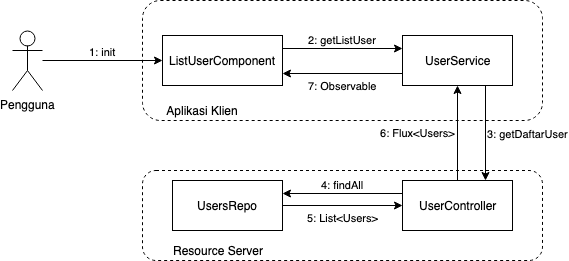
\includegraphics[width=1\textwidth]{./resources/comm-dia-list-user}
		\caption{Diagram \textit{Communication} Untuk Proses Menampilkan Data Pengguna}
		\label{fig:comm-dia-list-user}
	\end{figure}
	
	Prosesnya akan berlangsung seperti skenario di bawah ini :
	
	\begin{enumerate}
		\item Pengguna (\textit{resource owner}) akan melakukan akses ke menu daftar pengguna.
		\item Dari komponen \texttt{ListUserComponent} melakukan akses ke \texttt{UserService} untuk mendapatkan daftar pengguna.
		\item Komponen \texttt{UserService} melakukan akses ke \texttt{UserController} di \textit{Resource Server}.
		\item Kelas \textit{UserController} akan melakukan akses ke sistem basis data melalui \textit{UsersRepo} untuk mendapatkan daftar pengguna.
		\item Komponen \texttt{UsersRepo} akan mengembalikan daftar pengguna (\textit{user agent}) ke \texttt{UserController}.
		\item \texttt{UserController} akan memberikan \textit{response} ke aplikasi klien (\textit{user agent}) dalam bentuk JSON dimana transfer datanya akan bersifat \textit{asynchronuous}.
		\item Komponen \texttt{UserService} akan mengirimkan data ke ke \texttt{ListUserComponent} untuk ditampilkan dalam sebuah tabel.
	\end{enumerate}
	
	\item Fitur Tambah Pengguna Baru
	
	Diagram \textit{communication} untuk fitur ini menjelaskan proses yang terjadi pada saat pengguna menggunakan fitur tambah pengguna dari aplikasi klien (\textit{user agent}). Berikut adalah diagramnya :
	
	\begin{figure}[H]
		\centering
		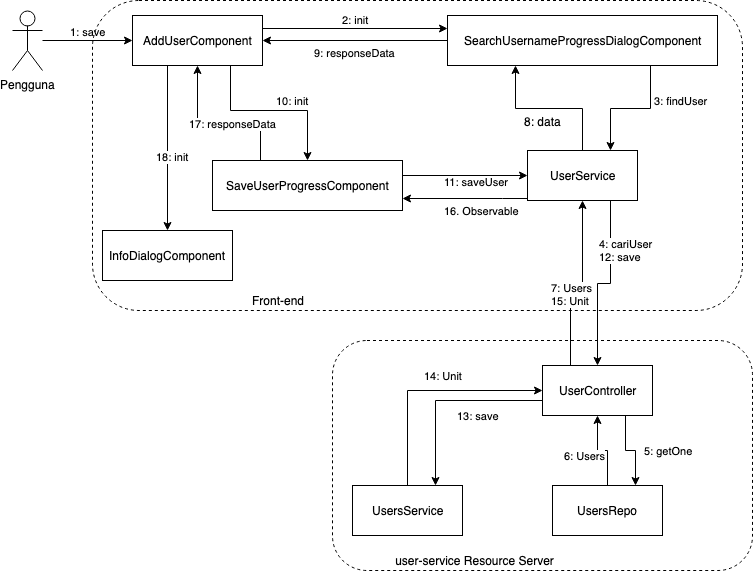
\includegraphics[width=1\textwidth]{./resources/comm-dia-add-user}
		\caption{Diagram \textit{Communication} Untuk Proses Tambah Data Pengguna}
		\label{fig:comm-dia-add-user}
	\end{figure}
	
	Proses komunikasi antar komponen untuk fitur ini akan terjadi seperti skenario berikut :
	
	\begin{enumerate}
		%1
		\item Pengguna melakukan aksi simpan data pengguna
		%2
		\item Komponen \texttt{AddUserComponent} akan melakukan pemanggilan komponen lain, yaitu \texttt{SearchUsernameProgressDialogComponent}
		%3
		\item Komponen \texttt{SearchUsernameProgressDialogComponent} akan melakukan permintaan data ke komponen \texttt{UserService}.
		%4
		\item \texttt{UserService} akan melakukan \textit{request} ke \textit{Resource Server} melalui \texttt{UserController}.
		%5
		\item \texttt{UserController} melakukan akses ke basis data melalui \texttt{UserRepo}
		%6
		\item \texttt{UserRepo} mengembalikan informasi detail dari pengguna yang diminta
		%7
		\item \texttt{UserController} memberikan \textit{response} ke \textit{front-end}, dalam hal ini adalah \texttt{UserService} berupa informasi detail pengguna
		%8
		\item \texttt{UserService} akan memberikan data ke \texttt{SearchUsernameProgressDialogComponent}.
		%9
		\item \texttt{SearchUsernameProgressDialogComponent} akan memberikan \textit{response} ke \texttt{AddUserComponent} bahwa data tersebut ada atau tidak ada, terdaftar atau belum terdaftar.
		%10
		\item Bila data pengguna belum pernah terdaftar sebelumnya, \texttt{AddUserComponent} akan melakukan pemanggilan ke komponen \texttt{SaveUserProgressComponent}
		%11
		\item \texttt{SaveUserProgressComponent} akan mengirimkan data ke \texttt{UserService} untuk dikirimkan ke \textit{resource server}.
		%12
		\item \texttt{UserService} melakukan \textit{request} ke \textit{resource server} melalui \texttt{UserController} dan mengirimkan data pengguna untuk disimpan dalam basis data.
		%13 
		\item \texttt{UserController} kemudian mengirimkan data pengguna yang akan disimpan ke basis data melalui \texttt{UserService}.
		%14
		\item \texttt{UsersService} akan mengirimkan informasi ke \texttt{UserController} bahwa data telah tersimpan.
		%15
		\item \texttt{UserController} akan mengirimkan \textit{response} ke \textit{front-end} bahwa data telah sukses tersimpan.
		%16
		\item \texttt{UserService} akan mengirimkan informasi suksesnya ke komponen \texttt{SaveUserProgressComponent}
		%17
		\item Dari \texttt{SaveUserProgressComponent} mengirimkan statusnya ke \texttt{AddUserComponent}.
		\item Kemudian \texttt{AddUserComponent} melakukan pemanggilan ke \texttt{InfoDialogComponent} untuk memberitahu pengguna (\textit{resource owner}) bahwa data telah tersimpan.
	\end{enumerate}
	
	\item Fitur Ubah Detail Pengguna
	
	Diagram \textit{communication} untuk fitur ini menjelaskan proses yang terjadi pada saat pengguna menggunakan fitur ubah data pengguna dari aplikasi klien (\textit{user agent}). Berikut adalah diagramnya :
	
	\begin{figure}[H]
		\centering
		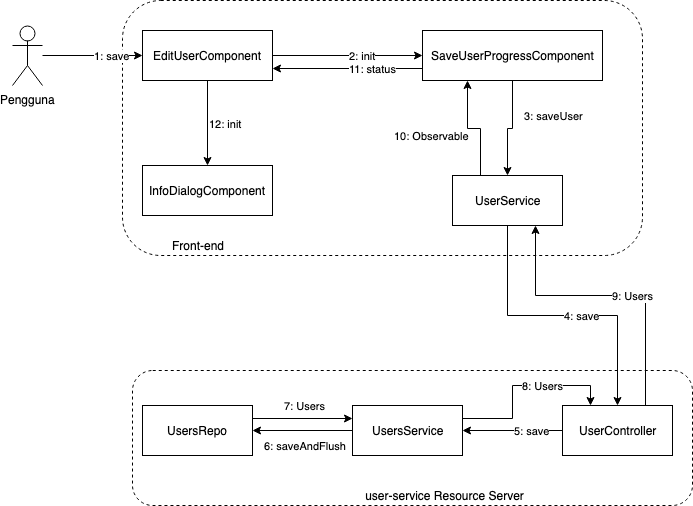
\includegraphics[width=1\textwidth]{./resources/comm-dia-update-user}
		\caption{Diagram \textit{Communication} Untuk Proses Ubah Data Pengguna}
		\label{fig:comm-dia-update-user}
	\end{figure}
	
	Penjelasan dari diagram tersebut adalah seperti berikut ini :
	
	\begin{enumerate}
	%1
		\item Pengguna melakukan simpan data melalui \texttt{EditUserComponent}
		%2
		\item Komponen \texttt{EditUserComponent} membuka komponen \texttt{SaveUserProgressComponent}
		%3
		\item Komponen \texttt{SaveUserProgressComponent} melakukan pemanggilan fungsi \texttt{saveUser} milik kelas \texttt{UserService}.
		%4
		\item \texttt{UserService} melakukan \textit{request} ke \textit{resource server}, dalam hal ini melalui \texttt{UserController} dengan mengirimkan data hasil perubahan yang telah dilakukan pengguna (\textit{resource owner}).
		%5
		\item \texttt{UserController} melakukan pemanggilan fungsi \texttt{save} milik kelas \texttt{UsersService} untuk melakukan pengolahan data.
		%6
		\item \texttt{UsersService} melakukan pemanggilan \textit{method} \texttt{saveAndFlush} milik \texttt{UsersRepo} sehingga data terbaru akan tersimpan dalam sistem basis data.
		%7
		\item \texttt{UsersRepo} setelah melakukan simpan data akan mengembalikan sebuah nilai dalam objek \texttt{Users} ke \texttt{UsersService}.
		%8
		\item Objek \texttt{Users} akan dikembalikan oleh \texttt{UsersService} ke \texttt{UserController} untuk nantinya dikirimkan ke aplikasi klien (\textit{user agent})
		%9
		\item \texttt{UserController} melakukan \textit{response} ke aplikasi klien (\textit{user agent}) dengan mengirimkan objek \texttt{Users} dalam bentuk JSON, kembali ke \texttt{UserService}.
		%10
		\item \texttt{UserService} akan mengirimkan data ke \texttt{SaveUserProgressComponent} dalam bentuk \texttt{Observable}
		%11
		\item \texttt{SaveUserProgressComponent} akan mengirimkan status keberhasilan proses simpan perubahan data pengguna ke \texttt{EditUserComponent}.
		%12
		\item \texttt{EditUserComponent} akan memanggil \texttt{InfoDialogComponent} untuk menampilkan informasi ke pengguna (\texttt{resource owner}) bahwa data telah tersimpan atau gagal disimpan.
	\end{enumerate}
	
	%05
	\item Fitur Hapus Pengguna
	
	Diagram \textit{communication} untuk fitur ini menjelaskan proses yang terjadi saat pengguna menggunakan fitur hapus data pengguna dari aplikasi klien (\textit{user agent}). Berikut adalah diagramnya :
	
	\begin{figure}[H]
		\centering
		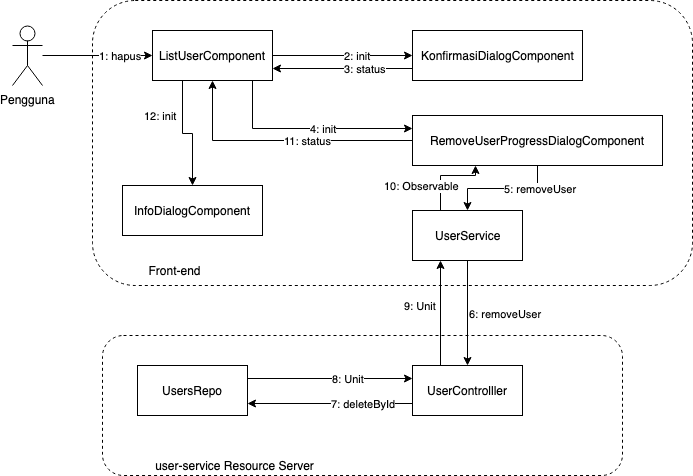
\includegraphics[width=1\textwidth]{./resources/comm-dia-hapus-user}
		\caption{Diagram \textit{Communication} Untuk Proses Hapus Data Pengguna}
		\label{fig:comm-dia-hapus-user}
	\end{figure}
	
	Penjelasan dari diagram tersebut adalah seperti berikut ini :
	
	\begin{enumerate}
		%1
		\item Pengguna (\textit{resource owner}) melakukan hapus data dari \texttt{ListUserComponent}.
		
		%2
		\item \texttt{ListUserComponent} memanggil komponen \texttt{KonfirmasiDialogComponent} untuk memastikan bahwa pengguna (\textit{resource owner}) melakukannya dengan sengaja.
		
		%3
		\item \texttt{KonfirmasiDialogComponent} mengirimkan jawaban dari pengguna (\textit{resource owner}) atas keputusannya untuk menghapus data.
		
		%4
		\item Komponen \texttt{ListUserComponent} memanggil \texttt{RemoveUserProgressDialogComponent}
		
		%5
		\item \texttt{RemoveUserProgressDialogComponen} memanggil \textit{method} \texttt{removeUser} milik \texttt{UserService}.
		
		%6
		\item \texttt{UserService} melakukan \textit{request} ke \textit{resource server}, dalam hal ini melalui \textit{method} \texttt{removeUser} milik kelas \texttt{UserController}.
		
		%7
		\item \texttt{UserController} memanggil \textit{method} \texttt{deleteById} milik \texttt{UsersRepo} untuk melakukan hapus data di sistem basis data 
		
		%8 
		\item \texttt{UsersRepo} melakukan hapus data dan mengembalikan nilai \texttt{Unit} yang sebetulnya tidak memiliki nilai apapun.
		
		%9
		\item \texttt{UserController} mengirimkan \textit{response} ke \textit{front-end} melalui \texttt{UserService}.
		
		%10
		\item \texttt{UserService} mengembalikan hasil ke \texttt{RemoveUserProgressDialogComponent} dalam bentuk \texttt{Observable}.
		
		%11
		\item \texttt{RemoveUserProgressDialogComponent} mengembalikan status ke \texttt{ListUserComponent} bahwa data telah terhapus.
		
		%12
		\item \texttt{ListUserComponent} memanggil \texttt{InfoDialogComponent} untuk memberitahu pengguna (\textit{resource owner}) bahwa data yang diinginkan telah dihapus
	\end{enumerate}
	
	%06
	\item Fitur Tampilkan Daftar Hak Akses
	
	Diagram \textit{communication} untuk fitur ini menjelaskan proses yang terjadi pada saat pengguna menggunakan fitur untuk menampilkan seluruh hak akses (\textit{role}) yang telah terdaftar melalui aplikasi klien (\textit{user agent}). Berikut adalah diagramnya :
	
	\begin{figure}[H]
		\centering
		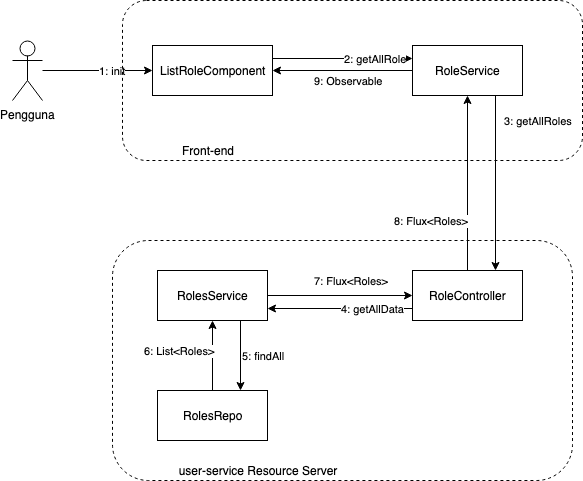
\includegraphics[width=1\textwidth]{./resources/comm-dia-list-role}
		\caption{Diagram \textit{Communication} Untuk Proses Menampilkan Daftar Hak Akses}
		\label{fig:comm-dia-list-role}
	\end{figure}
	
	Penjelasan dari diagram tersebut adalah seperti berikut ini :
	
	\begin{enumerate}
		%1
		\item Pengguna (\textit{resource owner}) melakukan akses ke fitur tampilkan daftar hak akses (\textit{role}) melalui komponen \texttt{ListRoleComponent}.
		
		%2
		\item \texttt{ListRoleComponent} memanggil \textit{method} \texttt{getAllRole()} milik \texttt{RoleService}
		
		%3
		\item \texttt{RoleService} melakukan \textit{request} ke \textit{resource server} melalui \textit{method} \texttt{getAllRoles()} milik kelas \texttt{RoleController}
		
		%4
		\item \texttt{RoleController} melakukan pemanggilan \textit{method} \texttt{getAllData()} milik kelas \texttt{RolesService}
		
		%5
		\item \texttt{RolesService} melakukan pemanggilan \textit{method} \texttt{findAll()} milik \texttt{RolesRepo} untuk mengambil daftar hak akses dari sistem basis data.
		
		%6
		\item \texttt{RolesRepo} mengembalikan daftar hak akses dalam bentuk \texttt{List<Roles>} ke \texttt{RolesService}
		
		%7
		\item \texttt{RolesService} mengembalikan nilai ke \texttt{RoleController} dalam bentuk \texttt{Flux<Roles>} yang menggunakan fitur \textit{reactive}
		
		%8
		\item \texttt{RoleController} akan memberikan \textit{response} ke \textit{front-end} berupa \texttt{Flux<Roles>} dalam bentuk JSON, untuk kasus ini, data akan dikirimkan ke \texttt{RoleService}.
		
		%9
		\item \texttt{RoleService} akan mengirimkan data ke \texttt{ListRoleComponent} dalam bentuk \texttt{Observable} yang kemudian datanya ditampilkan dalam tabel.
	\end{enumerate}
	
	%07
	\item Fitur Tambah Hak Akses Baru
	
	Diagram \textit{communication} untuk fitur ini menjelaskan proses yang terjadi pada saat pengguna menggunakan fitur tambah hak akses baru (\textit{role}) yang ada pada aplikasi klien (\textit{user agent}). Berikut adalah diagramnya :
	
	\begin{figure}[H]
		\centering
		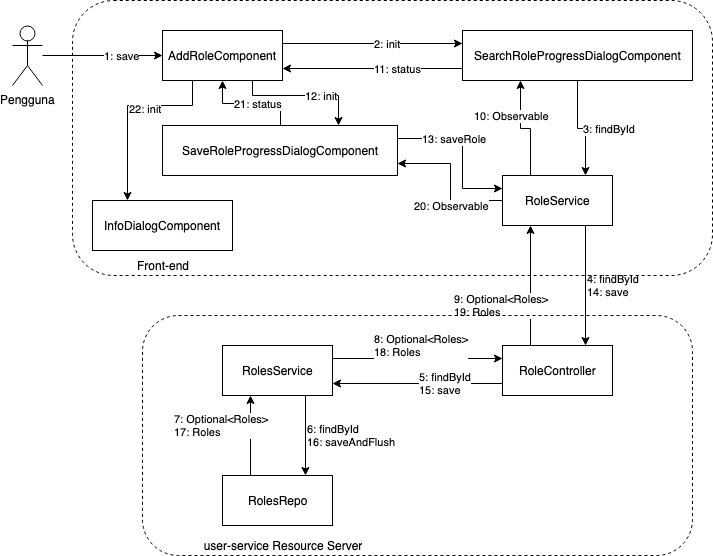
\includegraphics[width=1\textwidth]{./resources/comm-dia-add-role}
		\caption{Diagram \textit{Communication} Untuk Proses Tambah Data Hak Akses}
		\label{fig:comm-dia-add-role}
	\end{figure}
	
	Penjelasan untuk diagram tersebut adalah seperti berikut ini :
	
	\begin{enumerate}
		%1
		\item Pengguna (\textit{resource owner}) melakukan aksi simpan data di komponen \texttt{AddRoleComponent}
		
		%2
		\item \texttt{AddRoleComponent} mengaktifkan \texttt{SearchRoleProgressDialogComponent} untuk memeriksa apakah hak akses sudah pernah terdaftar dengan nama tersebut 
		
		%3
		\item \texttt{SearchRoleProgressDialogComponent} melakukan akses ke \textit{method} \texttt{findById()} milik \texttt{RoleService}
		
		%4
		\item \texttt{RoleService} melakukan \textit{request} ke \textit{resource server}, dalam hal ini melalui \textit{method} \texttt{findById} milik kelas \texttt{RoleController}
		
		%5
		\item \texttt{RoleController} melakukan pemanggilan \textit{method} \texttt{findById()} milik kelas \texttt{RolesService}
		
		%6
		\item \texttt{RolesService} melakukan pemanggilan \textit{method} \texttt{findById()} milik \texttt{RolesRepo} untuk melakukan simpan data ke sistem basis data.
		
		%7 
		\item \texttt{RolesRepo} setelah melakukan simpan data ke sistem basis data, akan mengembalikan respon berbentuk \texttt{Optional<Roles>} ke \texttt{RolesService}
		
		%8
		\item \texttt{RolesService} meneruskan pesan ke \texttt{RoleController} dalam bentuk yang sama, yaitu \texttt{Optional<Roles>}
		
		%9
		\item \texttt{RoleController} memberikan \textit{response} ke \textit{front-end}, dalam hal ini melalui \texttt{RoleService} berupa data \texttt{Optional<Roles>} dalam bentuk JSON.
		
		%10
		\item \texttt{RoleService} mengembalikan nilai ke \texttt{SearchRoleProgressDialogComponent} dalam bentuk \texttt{Observable}
		
		%11
		\item \texttt{SearchRoleProgressDialogComponent} mengembalikan status datanya apakah sudah terdaftar atau belum ke \texttt{AddRoleComponent}
		
		%12
		\item \texttt{AddRoleComponent} melakukan pemanggilan ke \texttt{SaveRoleProgressDialogComponent} untuk melakukan simpan data.
		
		%13
		\item \texttt{SaveRoleProgressDialogComponent} melakukan pemanggilan \textit{method} \texttt{saveRole()} milik \texttt{RoleService} untuk melakukan simpan data hak akses baru
		
		%14
		\item \texttt{RoleService} melakukan \textit{request} ke \textit{resource server} melalui \textit{method} \texttt{save} milik kelas \texttt{RoleController}
		
		%15
		\item \texttt{RoleController} melakukan akses terhadap \textit{method} \texttt{save} milik kelas \texttt{RolesService}
		
		%16
		\item \texttt{RolesService} melakukan simpan data dengan memanggil \textit{method} \texttt{saveAndFlush()} milik \texttt{RolesRepo}
		
		%17
		\item Setelah data tersimpan dalam sistem basis data, \texttt{RolesRepo} akan mengembalikan objek dari \texttt{Roles} ke \texttt{RolesService}
		
		%18
		\item \texttt{RolesService} meneruskan nilai yang berupa objek dari \texttt{Roles} ke \texttt{RoleController}
		
		%19
		\item \texttt{RoleController} memberikan \textit{response} berupa objek \texttt{Roles} dalam bentuk JSON ke \texttt{RoleService} di \textit{front-end}
		
		%20
		\item \texttt{RoleService} akan mengembalikan nilai dalam bentuk \texttt{Observable} ke \texttt{SaveRoleProgressDialogComponent}
		
		%21
		\item \texttt{SaveRoleProgressDialogComponent} memberikan status ke \texttt{AddRoleComponent} apakah datanya tersimpan atau tidak
		
		%22
		\item \texttt{AddRoleComponent} mengaktifkan \texttt{InfoDialogComponent} sebagai informasi bagi pengguna (\textit{resource owner}) apakah datanya telah berhasil tersimpan atau gagal.
	\end{enumerate}
	
	%08
	\item Fitur Ubah Hak Akses
	
	Diagram \textit{communication} untuk fitur ini menjelaskan proses yang terjadi pada saat pengguna (\textit{resource owner}) menggunakan fitur ubah data hak akses (\textit{role}) yang ada pada aplikasi klien (\textit{user agent}). Berikut adalah diagramnya :
	
	\begin{figure}[H]
		\centering
		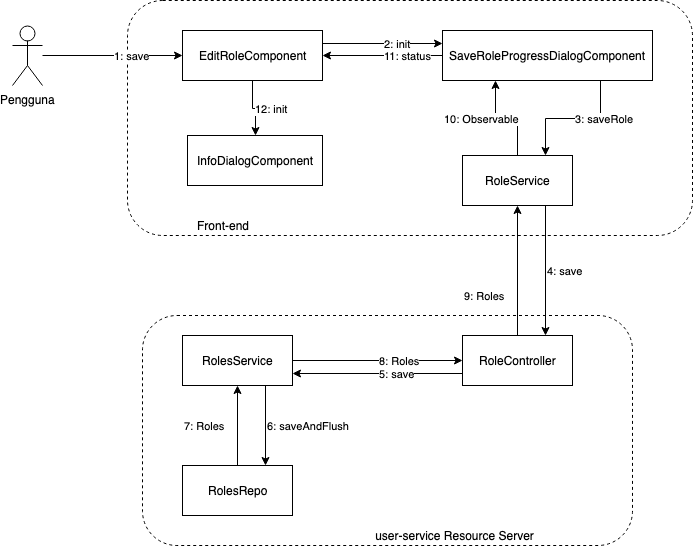
\includegraphics[width=1\textwidth]{./resources/comm-dia-edit-role}
		\caption{Diagram \textit{Communication} Untuk Proses Ubah Data Hak Akses}
		\label{fig:comm-dia-edit-role}
	\end{figure}
	
	Penjelasan untuk diagram tersebut adalah seperti berikut ini :
	
	\begin{enumerate}
		%1
		\item Pengguna (\textit{resource owner}) melakukan simpan data perubahan melalui \texttt{EditRoleComponent}
		
		%2
		\item \texttt{EditRoleComponent} memanggil komponen \texttt{SaveRoleProgressDialogComponent} untuk menunjukkan ke pengguna (\textit{resource owner}) bahwa proses simpan data sedang berjalan.
		
		%3
		\item \texttt{SaveRoleProgressDialogComponent} melakukan akses ke \textit{method} \texttt{saveRole} milik \texttt{RoleService} dengan membawa data hasil perubahan
		
		%4
		\item \texttt{RoleService} melakukan \textit{request} ke \textit{resource server}, dalam hal ini melalui \textit{method} \texttt{save} milik kelas \texttt{RoleController}
		
		%5
		\item \texttt{RoleController} memanggil \textit{method} \texttt{save} milik kelas \texttt{RolesService}
		
		%6
		\item \texttt{RolesService} akan memanggil \textit{method} \texttt{saveAndFlush} milik \texttt{RolesRepo} untuk kemudian disimpan dalam sistem basis data 
		
		%7
		\item \texttt{RolesRepo} setelah melakukan simpan data ke sistem basis data, akan mengembalikan sebuah objek \texttt{Roles} ke \texttt{RolesService}
		
		%8
		\item \texttt{RolesService} akan meneruskan objek \texttt{Roles} ke \texttt{RoleController}
		
		%9
		\item \texttt{RoleController} melakukan \textit{response} ke \textit{front-end} melalui \texttt{RoleService} yang sebelumnya melakukan \textit{request}.
		
		%10
		\item \texttt{RoleService} mengirimkan data dari \textit{response} \textit{resource server} ke \texttt{SaveRoleProgressDialogComponent} dalam bentuk \texttt{Observable}
		
		%11
		\item \texttt{SaveRoleProgressDialogComponent} mengirimkan status ke \texttt{EditRoleComponent} sebagai tanda apakah simpan data berhasil dilakukan atau gagal.
		
		%12
		\item \texttt{EditRoleComponent} melakukan pemanggilan \texttt{InfoDialogComponent} untuk memberitahu pengguna (\textit{resource server}) bahwa data berhasil tersimpan atau gagal.
	\end{enumerate}
	
	%09
	\item Fitur Hapus Hak Akses
	
	Diagram \textit{communication} untuk fitur ini menjelaskan proses yang terjadi pada saat pengguna (\textit{resource owner}) menggunakan fitur hapus data hak akses (\textit{role}) yang ada pada aplikasi klien (\textit{user agent}). Berikut adalah diagramnya :
	
	\begin{figure}[H]
		\centering
		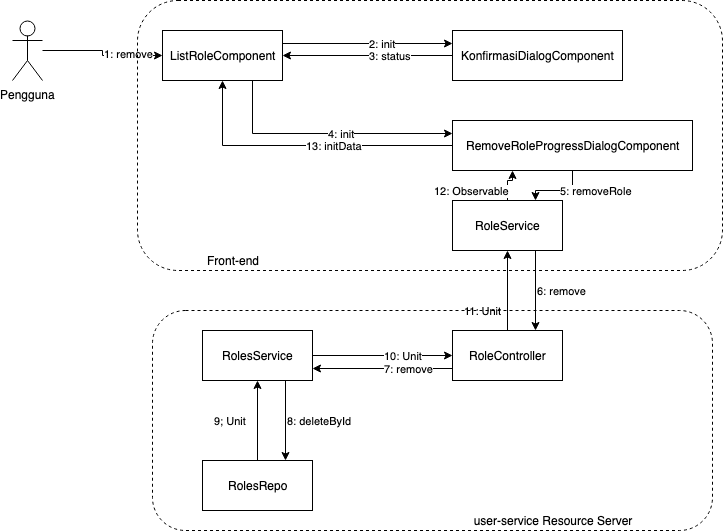
\includegraphics[width=1\textwidth]{./resources/comm-dia-remove-role}
		\caption{Diagram \textit{Communication} Untuk Proses Hapus Data Hak Akses}
		\label{fig:comm-dia-remove-role}
	\end{figure}
	
	Penjelasan diagram tersebut adalah seperti berikut ini :
	
	\begin{enumerate}
		%1
		\item Pengguna (\textit{resource owner}) melakukan hapus data hak akses melalui \texttt{ListRoleComponent}
		
		%2
		\item \texttt{ListRoleComponent} melakukan pemanggilan \texttt{KonfirmasiDialogComponent} untuk memastikan bahwa pengguna (\textit{resource owner}) benar-benar melakukan permintaan hapus data hak akses
		
		%3
		\item \texttt{KonfirmasiDialogComponent} mengembalikan status pilihan pengguna (\textit{resource owner}) ke \texttt{ListRoleComponent} bahwa data benar akan dihapus atau tidak
		
		%4
		\item \texttt{ListRoleComponent} akan mengaktifkan \texttt{RemoveRoleProgressDialogComponent} untuk melakukan proses hapus data hak akses
		
		%5
		\item \texttt{RemoveRoleProgressDialogComponent} melakukan akses ke fungsi \texttt{removeRole} milik \texttt{RoleService}
		
		%6
		\item \texttt{RoleService} melakukan \textit{request} ke \textit{resource server} melalui \textit{method} \texttt{remove} milik kelas \texttt{RoleController}
		
		%7
		\item \texttt{RoleController} melakukan akses ke \textit{method} \texttt{remove} milik kelas \texttt{RolesService}
		
		%8
		\item \texttt{RolesService} melakukan akses ke \textit{method} \texttt{deleteById} milik \texttt{RolesRepo} untuk menghapus data hak akses pada sistem data
		
		%9
		\item Setelah \texttt{RolesRepo} menghapus data hak akses pada sistem data, \texttt{RolesRepo} mengembalikan nilai kosong dalam bentuk \texttt{Unit} ke \texttt{RolesService}
		
		%10
		\item \texttt{RolesService} akan meneruskan hasil nilai \texttt{Unit} ke \texttt{RoleController}
		
		%11
		\item \texttt{RoleController} akan memberikan \textit{response} berupa \texttt{Unit} ke \textit{front-end} melalui kelas \texttt{RoleService} yang sebelumnya melakukan \textit{request}.
		
		%12
		\item \texttt{RoleService} akan mengembalikan nilai ke \texttt{RemoveRoleProgressDialogComponent} dalam bentuk \texttt{Observable}
		
		%13
		\item \texttt{RemoveROleProgressDialogComponent} akan mengembalikan nilai ke \texttt{ListRoleComponent} untuk melakukan \textit{refresh} tabel daftar hak akses
	\end{enumerate}
	
	%10
	\item Fitur Tampilkan Daftar Pengguna Dengan Hak Akses
	
	Diagram \textit{communication} untuk fitur ini menjelaskan proses yang terjadi pada saat pengguna (\textit{resource owner}) melakukan akses terhadap daftar hak akses yang diberikan ke pengguna yang terdaftar. Diagramnya akan terlihat seperti berikut :
	
	\begin{figure}[H]
		\centering
		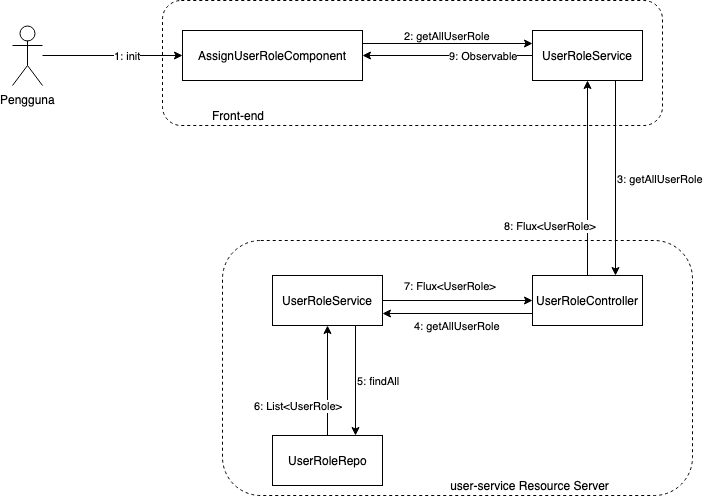
\includegraphics[width=1\textwidth]{./resources/comm-dia-list-user-role}
		\caption{Diagram \textit{Communication} Untuk Melihat Daftar Hak Akses Yang Diberikan Ke Pengguna}
		\label{fig:comm-dia-list-user-role}
	\end{figure}
	
	Penjelasan dari diagram tersebut adalah seperti berikut ini :
	
	\begin{enumerate}
		%1
		\item Pengguna melakukan akses ke daftar hak akses yang diberikan ke pengguna melalui \texttt{AssignUserRoleComponent}
		
		%2
		\item \texttt{AssignUserRoleComponent} melakukan akses ke fungsi \texttt{getAllUserRole} ke \texttt{UserRoleService}
		
		%3
		\item \texttt{UserRoleService} melakukan \textit{request} ke \textit{resource server} melalui \textit{method} \texttt{getAllUserRole} milik kelas \texttt{UserRoleController}
		
		%4
		\item \texttt{UserRoleController} melakukan akses ke \textit{method} \texttt{getAllUserRole} milik \texttt{UserRoleService}
		
		%5
		\item \texttt{UserRoleService} melakukan akses ke \textit{method} \texttt{findAll} milik \texttt{UserRoleRepo} untuk mengambil seluruh data hak akses yang diberikan ke pengguna yang tercatat dalam sistem basis data
		
		%6
		\item \texttt{UserRoleRepo} mengembalikan nilai ke \texttt{UserRoleService} dalam bentuk \texttt{List<UserRole>}
		
		%7
		\item \texttt{UserRoleService} mengembalikan nilai ke \texttt{UserRoleController} dalam bentuk \texttt{Flux<UserRole>}
		
		%8
		\item \texttt{UserRoleController} memberikan \textit{response} ke bagian \textit{front-end} melalui \texttt{UserRoleService} yang sebelumnya melakukan \textit{request} dalam bentuk \texttt{Flux<UserRole>}
		
		%9
		\item \texttt{UserRoleService} akan memberikan nilai ke \texttt{AssignUserRoleComponent} dalam bentuk \texttt{Observable} untuk kemudian ditampilkan dalam tabel
	\end{enumerate}
	
	%11
	\item FItur Tambahkan Hak Akses ke Pengguna
	
	Diagram \textit{communication} untuk fitur ini menjelaskan proses yang terjadi pada saat pengguna (\textit{resource owner}) melakukan penambahan data hak akses untuk pengguna yang terdaftar. Diagramnya akan terlihat seperti berikut :
	
	\begin{figure}[H]
		\centering
		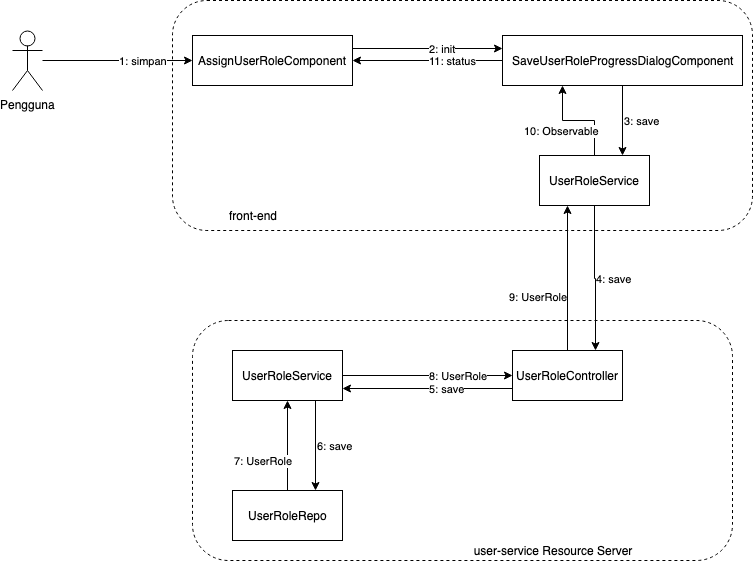
\includegraphics[width=1\textwidth]{./resources/comm-dia-add-user-role}
		\caption{Diagram \textit{Communication} Untuk Menambahkan Data Hak Akses Bagi Pengguna}
		\label{fig:comm-dia-add-user-role}
	\end{figure}
	
	Penjelasan diagram di atas adalah seperti berikut :
	
	\begin{enumerate}
		%1
		\item Pengguna (\textit{resource owner}) melakukan simpan data dari hak akses yang diberikan ke pengguna melalui \texttt{AssignUserRoleComponent}.
		
		%2
		\item \texttt{AssignUserRoleComponent} melakukan pemanggilan ke \texttt{SaveUserRoleProgressDialogComponent}
		
		%3
		\item \texttt{SaveUserRoleProgressDialogComponent} melakukan akses ke \textit{method} \texttt{save} milik \texttt{UserRoleService}
		
		%4
		\item \texttt{UserRoleService} melakukan \textit{request} ke \textit{resource server} melalui \textit{method} \texttt{save} milik \texttt{UserRoleController} dengan membawa informasi data hak akses yang diberikan ke pengguna (\textit{resource owner}).
		
		%5
		\item \texttt{UserRoleController} melakukan akses ke \textit{method} \texttt{save} milik \texttt{UserRoleService}
		
		%6 
		\item \texttt{UserRoleService} melakukan akses ke \textit{method} \texttt{save} milik \texttt{UserRoleRepo} untuk menyimpan data ke sistem basis data
		
		%7
		\item \texttt{UserRoleRepo} setelah melakukan simpan data ke sistem basis data akan mengembalikan nilai berupa objek dari \texttt{UserRole} ke \texttt{UserRoleService}
		
		%8
		\item \texttt{UserRoleService} meneruskan nilai dari objek \texttt{UserRole} ke \texttt{UserRoleController}
		
		%9 
		\item \texttt{UserRoleController} akan memberikan \textit{response} ke \textit{front-end} berupa objek dari kelas \texttt{UserRole} atas \textit{request} yang sebelumnya dilakukan oleh \texttt{UserRoleService}
		
		%10
		\item \texttt{UserRoleService} akan mengembalikan nilai ke \texttt{SaveUserRoleProgressDialogComponent} dalam bentuk \texttt{Observable}
		
		%11
		\item \texttt{SaveUserRoleProgressDialogComponent} akan mengembalikan sebuah status ke \texttt{AssignUserRoleComponent} untuk kemudian \texttt{AssignUserRoleComponent} melakukan \textit{refresh} atau pembaruan pada tabel daftar hak akses yang telah diberikan ke pengguna
	\end{enumerate}
	
	%12
	\item Fitur Hapus Hak Akses dari Pengguna
	
	Diagram \textit{communication} untuk fitur ini menjelaskan proses yang terjadi pada saat pengguna (\textit{resource owner}) melakukan penghapusan data hak akses yang telah diberikan ke pengguna yang terdaftar. Diagramnya akan terlihat seperti berikut :
	
	\begin{figure}
		\centering
		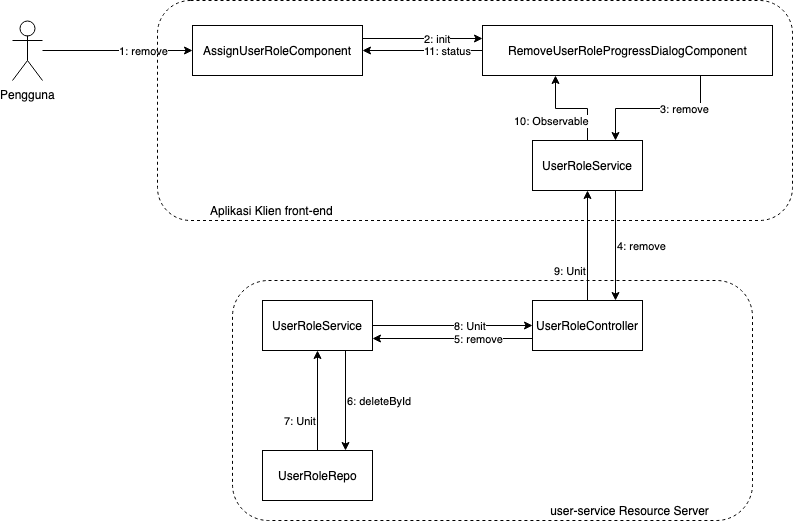
\includegraphics[width=1\textwidth]{./resources/comm-dia-remove-user-role}
		\caption{Diagram \textit{Communication} Untuk Menghapus Data Hak Akses Yang Telah Diberikan Ke Pengguna}
		\label{fig:comm-dia-remove-user-role}
	\end{figure}
	
	Penjelasan dari diagram tersebut adalah seperti berikut ini :
	
	\begin{enumerate}
		%1
		\item Pengguna (\textit{resource owner}) melakukan akses hapus data hak akses untuk pengguna yang telah terdaftar melalui \texttt{AssignUserRoleComponent}
		
		%2
		\item \texttt{AssignUserRoleComponent} melakukan pemanggilan ke \texttt{RemoveUserRoleProgressDialogComponent} untuk melakukan proses penghapusan hak akses terhadap pengguna yang terpilih
		
		%3
		\item \texttt{RemoveUserRoleProgressDialogComponent} melakukan akses ke fungsi \texttt{remove} milik \texttt{UserRoleService}
		
		%4
		\item \texttt{UserRoleService} melakukan \textit{request} ke \textit{resource server} melalui \textit{method} \texttt{remove} milik kelas \texttt{UserRoleController}
		
		%5
		\item \texttt{UserRoleController} melakukan akses ke \textit{method} \texttt{remove} milik kelas \texttt{UserRoleService}
		
		%6
		\item \texttt{UserRoleService} melakukan akses ke \textit{method} \texttt{deleteById} milik \texttt{UserRoleRepo} untuk menghapus data hak akses milik pengguna yang terdaftar di sistem basis data
		
		%7
		\item Setelah melakukan hapus data di sistem basis data, \texttt{UserRoleRepo} mengembalikan respon berupa kelas \texttt{Unit} yang sebetulnya tidak ada nilainya.
		
		%8
		\item \texttt{UserRoleService} meneruskan respon berupa kelas \texttt{Unit} ke \texttt{UserRoleController}
		
		%9
		\item \texttt{UserRoleController} mengirimkan \textit{response} ke aplikasi klien berupa kelas \texttt{Unit} dalam bentuk JSON, dalam hal ini ke kelas \texttt{UserRoleService}
		
		%10
		\item \texttt{UserRoleService} meneruskan \textit{response} ke \texttt{RemoveUserRoleProgressDialogComponent} dalam bentuk \texttt{Observable}
		
		%11
		\item \texttt{RemoveUserRoleProgressDialogComponent} memberikan status ke \texttt{AssignUserRoleComponent} untuk melakukan \textit{refresh} tabel daftar hak akses untuk pengguna.
	\end{enumerate}
	
	%13
	\item Fitur Tampilkan Daftar Aplikasi Klien
	
	Diagram \textit{communication} untuk fitur ini menjelaskan proses yang terjadi pada saat pengguna (\textit{resource owner}) menggunakan fitur untuk melihat daftar aplikasi klien yang terdaftar. Diagramnya akan terlihat seperti berikut :
	
	\begin{figure}[H]
		\centering
		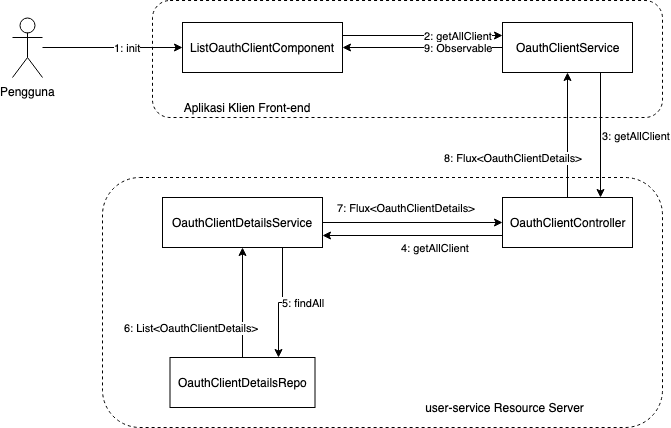
\includegraphics[width=1\textwidth]{./resources/comm-dia-list-client}
		\caption{Diagram \textit{Communication} Untuk Menampilkan Daftar Aplikasi Klien Yang Terdaftar}
		\label{fig:comm-dia-list-client}
	\end{figure}
	
	Penjelasan untuk diagram tersebut adalah seperti berikut :
	
	\begin{enumerate}
		%1
		\item Pengguna (\textit{resource owner}) melakukan akses ke fitur tampilkan daftar aplikasi klien melalui \texttt{ListOauthClientComponent}
		
		%2
		\item \texttt{ListOauthClientComponent} melakukan akses ke fungsi \texttt{getAllClient} milik kelas \texttt{OauthClientService}
		
		%3
		\item \texttt{OauthClientService} melakukan \textit{request} ke \textit{resource owner} melalui \textit{method} \texttt{getAllClient} milik kelas \texttt{OauthClientController}
		
		%4
		\item \texttt{OauthClientController} melakukan akses ke \textit{method} \texttt{getAllClient} milik \texttt{OauthClientDetailsService}
		
		%5
		\item \texttt{OauthClientDetailsService} melakukan akses ke \textit{method} \texttt{findAll} milik \texttt{OauthClientDetailsRepo} untuk melakukan akses ke sistem basis data.
		
		%6
		\item Setelah \texttt{OauthClientDetailsRepo} mengambil data dari sistem basis data, \texttt{OauthClientDetailsRepo} akan mengembalikan nilai berupa \texttt{List<OauthClientDetails>} yang berisi daftar aplikasi klien beserta detailnya.
		
		%7
		\item \texttt{OauthClientDetailsService} akan meneruskan data ke \texttt{OauthClientController} dalam bentuk objek dari \texttt{Flux<OauthClientDetails>}
		
		%8
		\item \texttt{OauthClientController} akan memberikan \textit{response} ke aplikasi klien berupa objek dari \texttt{Flux<OauthClientDetails>}, tentuna melalui \texttt{OauthClientService} karena sebelumnya melakukan \textit{request}
		
		%9
		\item \texttt{OauthClientService} mengembalikan nilai ke \textit{ListOauthClientComponent} untuk ditampilkan dalam tabel nantinya dalam bentuk \texttt{Observable}
	\end{enumerate}
	
	%14
	\item Fitur Tambah Aplikasi Klien
	
	Diagram \textit{communication} untuk fitur ini menjelaskan proses yang terjadi pada saat pengguna (\textit{resource owner}) menggunakan fitur untuk menambahkan aplikasi klien ke dalam sistem otentikasi. Diagramnya akan terlihat seperti berikut :
	
	\begin{figure}[H]
		\centering
		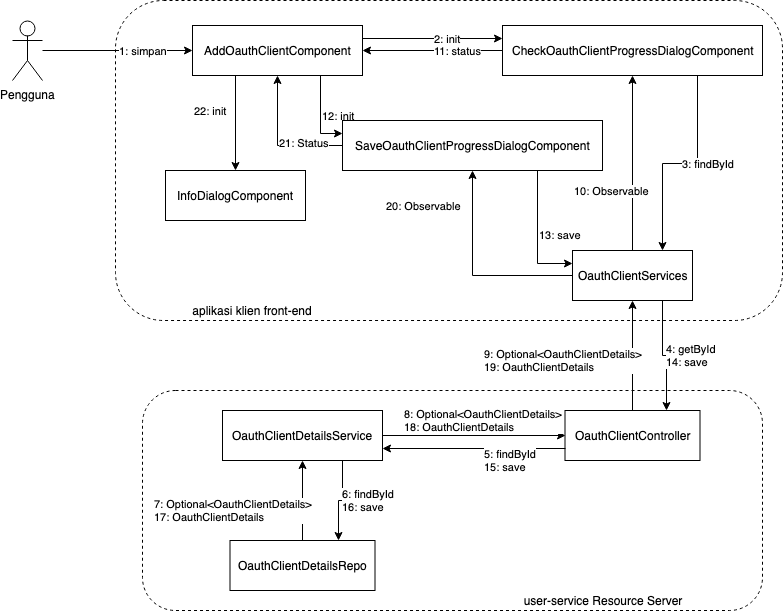
\includegraphics[width=1\textwidth]{./resources/comm-dia-add-client}
		\caption{Diagram \textit{Communication} Untuk Menambahkan Data Aplikasi Klien}
		\label{fig:comm-dia-add-client}
	\end{figure}
	
	Penjelasan dari diagram tersebut adalah sebagai berikut :
	
	\begin{enumerate}
		%1
		\item Pengguna (\textit{resource owner}) melakukan aksi simpan data aplikasi klien yang baru melalui \texttt{AddOauthClientComponent}
		
		%2
		\item \texttt{AddOauthClientComponent} melakukan pemanggilan ke \texttt{CheckOauthClientProgressDialogComponent} untuk melakukan pemeriksaan terhadap data yang akan disimpan, apakah datanya sudah ada dalam sistem basis data atau belum
		
		%3
		\item \texttt{CheckOauthClientProgressDialogComponent} melakukan akses ke fungsi \texttt{findById} milik \texttt{OauthClientServices}
		
		%4
		\item \texttt{OauthClientServices} melakukan \textit{request} ke \textit{resource server} melalui \textit{method} \texttt{getById} milik kelas \texttt{OauthClientController}
		
		%5
		\item \texttt{OauthClientController} melakukan akses ke \textit{method} \texttt{findById} milik \texttt{OauthClientDetailsService}
		
		%6
		\item \texttt{OauthClientDetailsService} melakukan akses ke \textit{method} \texttt{findById} milik \texttt{OauthClientDetailsRepo} untuk memeriksa apakah ada aplikasi klien dengan \textit{id} yang diminta, bila datanya ada, itu artinya aplikasi klien tersebut sebetulnya sudah terdaftar.
		
		%7
		\item Hasil dari akses ke sistem basis data, \texttt{OauthClientDetailsRepo} mengembalikan nilai ke \texttt{OauthClientDetailsService} dalam bentuk \texttt{Optional<OauthClientDetails>}
		
		%8
		\item \texttt{OauthClientDetailsService} meneruskan objek \texttt{Optional<OauthClientDetails>} ke \texttt{OauthClientController}
		
		%9
		\item \texttt{OauthClientController} memberikan \textit{response} ke aplikasi klien, dalam hal ini melalui \texttt{OauthClientServices} karena sebelumnya melakukan \textit{request} tersebut berupa objek \texttt{Optional<OauthClientDetails>} dalam bentuk JSON
		
		%10
		\item \texttt{OauthClientServices} meneruskan hasil \textit{response} yang dikirimkan oleh \textit{resource server} ke \texttt{CheckOauthClientProgressDialogComponent} dalam bentuk \texttt{Observable}
		
		%11
		\item \texttt{CheckOauthClientProgressDialogComponent} mengirimkan status ke \texttt{AddOauthClientComponent} yang memberikan informasi apakah data yang akan disimpan sudah pernah terrekam atau belum dalam basis data
		
		%12
		\item \texttt{AddOauthClientComponent} melakukan pemanggilan ke \texttt{SaveOauthClientProgressDialogComponent}
		
		%13
		\item \texttt{SaveOauthClientProgressDialogComponent} melakukan akses ke fungsi \texttt{save} milik \texttt{OauthClientServices}
		
		%14
		\item \texttt{OauthClientServices} melakukan \textit{request} ke \textit{resource server} melalui \textit{method} \texttt{save} milik kelas \texttt{OauthClientController}
		
		%15
		\item \texttt{OauthClientController} melakukan akses ke \texttt{OauthClientDetailsService} melalui \textit{method} \texttt{save}
		
		%16
		\item \texttt{OauthClientDetailsService} melakukan akses ke \textit{method} \texttt{save} milik \texttt{OauthClientDetailsRepo} untuk melakukan simpan data ke sistem basis data.
		
		%17
		\item Setelah melalui proses simpan data ke sistem basis data, \texttt{OauthClientDetailsRepo} mengembalikan nilai ke \texttt{OauthClientDetailsService} dalam bentuk objek \texttt{Optional<OauthClientDetails>}
		
		%18
		\item \texttt{OauthClientDetailsService} meneruskan objek \texttt{Optional<OauthClientDetails>} ke \texttt{OauthClientController}
		
		%19
		\item \texttt{OauthClientController} memberikan \textit{response} berupa \texttt{Optional<OauthClientDetails>} dalam bentuk JSON ke \textit{front-end}, dalam hal ini ke \texttt{OauthClientServices} yang sebelumnya melakukan \textit{request} ke \textit{resource server}
		
		%20
		\item \texttt{OauthClientServices} meneruskan hasil \textit{response} dari \textit{resource server} ke \texttt{SaveOauthClientProgressDialogComponent} dalam bentuk \texttt{Observable}
		
		%21
		\item \texttt{SaveOauthClientProgressDialogComponent} mengembalikan sebuah status ke \texttt{AddOauthClientComponent} sebagai tanda apakah datanya berhasil disimpan ke dalam basis data atau tidak
		
		%22
		\item \texttt{AddOauthClientComponent} memanggil \texttt{InfoDialogComponent} untuk memberitahu pengguna (\textit{resource owner}) bahwa data berhasil disimpan atau gagal disimpan.
	\end{enumerate}
	
	%15
	\item Fitur Ubah Detail Aplikasi Klien
	
	Diagram \textit{communication} untuk fitur ini menjelaskan proses yang terjadi pada saat pengguna (\textit{resource owner}) menggunakan fitur untuk mengubah detail dari data aplikasi klien yang telah terdaftar dalam sistem basis data. Diagramnya akan terlihat seperti berikut :
	
	\begin{figure}[H]
		\centering
		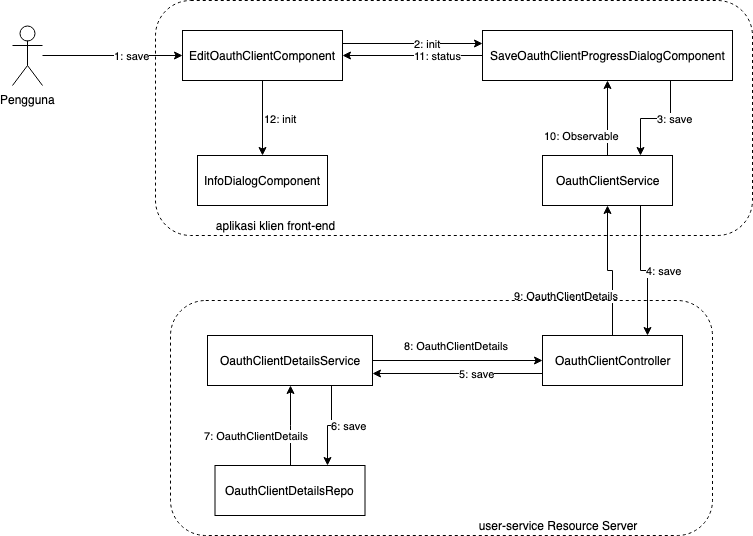
\includegraphics[width=1\textwidth]{./resources/comm-dia-edit-client}
		\caption{Diagram \textit{Communication} Untuk Mengubah Detail Data Aplikasi Klien}
		\label{fig:comm-dia-edit-client}
	\end{figure}
	
	Penjelasan dari diagram tersebut adalah seperti berikut :
	
	\begin{enumerate}
		%1
		\item Pengguna melakukan proses simpan terhadap perubahan data aplikasi klien dari \texttt{EditOauthClientComponent}
		
		%2
		\item \texttt{EditOauthClientComponent} memanggil \texttt{SaveOauthClientProgressDialogComponent} untuk memulai proses simpan perubahan data ke sistem basis data
		
		%3
		\item \texttt{SaveOauthClientProgressDialogComponent} melakukan akses ke fungsi \texttt{save} milik \texttt{OauthClientService}
		
		%4
		\item \texttt{OauthClientService} melakukan \textit{request} simpan data ke \textit{resource server} melalui \textit{method} \texttt{save} milik \texttt{OauthClientController}
		
		%5
		\item \texttt{OauthClientController} melakukan akses ke \textit{method} \texttt{save} milik \texttt{OauthClientDetailsService}
		
		%6 
		\item \texttt{OauthClientDetailsService} melakukan akses ke \textit{method} \texttt{save} milik \texttt{OauthClientDetailsRepo} untuk melakukan simpan data ke sistem basis data
		
		%7
		\item Setelah melakukan simpan data ke sistem basis data, \texttt{OauthClientDetailsRepo} mengirimkan objek \texttt{OauthClientDetails} ke \texttt{OauthClientDetailsService}
		
		%8
		\item \texttt{OauthClientDetailsService} meneruskan nilai berupa objek \texttt{OauthClientDetails} ke \texttt{OauthClientController}
		
		%9
		\item \texttt{OauthClientController} mengirimkan \textit{response} ke \textit{front-end} dalam hal ini adalah \texttt{OauthClientService} yang sebelumnya mengirimkan \textit{request} untuk simpan perubahan data aplikasi klien
		
		%10
		\item \texttt{OauthClientService} meneruskan hasil \textit{response} dari \textit{resource server} ke \texttt{SaveOauthClientProgressDialogComponent} dalam bentuk \texttt{Observable}
		
		%11
		\item \texttt{SaveOauthClientProgressDialogComponent} akan mengembalikan status ke \texttt{EditOauthClientComponent} apakah hasil perubahan data berhasil disimpan ke sistem basis data atau tidak.
		
		%12
		\item \texttt{EditOauthClientComponent} memanggil \texttt{InfoDialogComponent} untuk memberitahu pengguna (\textit{resource owner}) bahwa proses simpan data perubahan berhasil atau tidak.
	\end{enumerate}
	
	%16
	\item Fitur Hapus Aplikasi Klien
	
	Diagram \textit{communication} untuk fitur ini menjelaskan proses yang terjadi pada saat pengguna (\textit{resource owner}) menggunakan fitur untuk menghapus detail data dari aplikasi klien yang telah terdaftar dalam sistem basis data. Diagramnya akan terlihat seperti berikut :
	
	\begin{figure}[H]
		\centering
		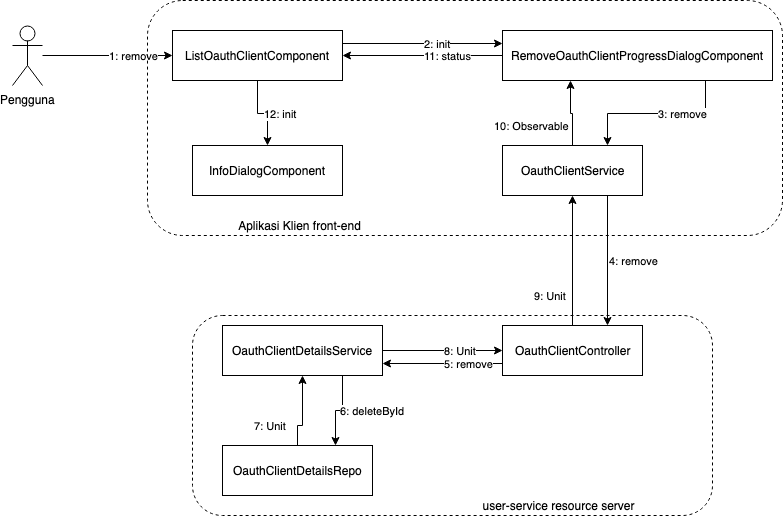
\includegraphics[width=1\textwidth]{./resources/comm-dia-remove-client}
		\caption{Diagram \textit{Communication} Untuk Menghapus Detail Data Aplikasi Klien}
		\label{fig:comm-dia-remove-client}
	\end{figure}
	
	Penjelasan dari diagram tersebut adalah seperti berikut ini :
	
	\begin{enumerate}
		%1
		\item Pengguna melakukan aksi hapus data aplikasi klien melalui \texttt{ListOauthClientComponent}
		
		%2
		\item \texttt{ListOauthClientComponent} memanggil \texttt{RemoveOauthClientProgressDialogComponent} untuk memulai proses hapus data aplikasi klien dan pengguna (\textit{resource owner}) mengetahui prosesnya masih berjalan
		
		%3
		\item \texttt{RemoveOauthClientProgressDialogComponent} melakukan akses ke fungsi \texttt{remove} milik \texttt{OauthClientService}
		
		%4
		\item \texttt{OauthClientService} melakukan \textit{request} ke \textit{resource server}, dalam hal ini melalui \textit{method} \texttt{remove} milik kelas \texttt{OauthClientController}
		
		%5
		\item \texttt{OauthClientController} melakukan akses ke \textit{method} \texttt{remove} milik \texttt{OauthClientDetailsService}
		
		%6
		\item \texttt{OauthClientDetailsService} melakukan akses ke \textit{method} \texttt{deleteById} milik \texttt{OauthClientDetailsRepo} agar data klien yang dimaksud terhapus dari sistem basis data.
		
		%7
		\item Setelah \texttt{OauthClientDetailsRepo} melakukan penghapusan data aplikasi klien di sisi sistem basis data, \texttt{OauthClientDetailsRepo} mengirimkan objek berupa \texttt{Unit} yang sebetulnya tidak ada nilainya.
		
		%8
		\item \texttt{OauthClientDetails Service} meneruskan objek \texttt{Unit} ke \texttt{OauthClientController}
		
		%9
		\item \texttt{OauthClientController} memberikan \textit{response} ke \textit{front-end} melalui \texttt{OauthClientService} karena sebelumnya melakukan \textit{request}
		
		%10
		\item \texttt{OauthClientService} meneruskan hasil \textit{response} ke \texttt{RemoveOauthClientProgressDialogComponent} dalam bentuk \texttt{Observable}
		
		%11
		\item \texttt{RemoveOauthClientProgressDialogComponent} memberikan sebuah status ke \texttt{ListOauthClientComponent} bahwa data berhasil dihapus atau tidak
		
		%12
		\item \texttt{ListOauthClientComponent} akan memanggil \texttt{InfoDialogComponent} untuk memberikan informasi kepada pengguna (\textit{resource owner}) bahwa data berhasil dihapus dari sistem basis data atau tidak.
	\end{enumerate}		
	
\end{itemize}

\subsubsection{Diagram \textit{Activity}}

Diagram ini masuk dalam kategori diagram \textit{behavior} yang menunjukkan alur kontrol atau alur objek yang dipertegas dalam urutan aktivitas dan kondisi pada alur yang terjadi. 

Seperti halnya diagram \textit{communication}, akan lebih mudah apabila diagram ini dibentuk dari beberapa skenario yang telah ditetapkan seperti berikut :

\begin{itemize}
	%1
	\item Diagram \textit{Activity} \textit{Login}
	
	Diagram \textit{activity} untuk kasus \textit{login} adalah seperti berikut :
	
	\begin{figure}[H]
		\centering
		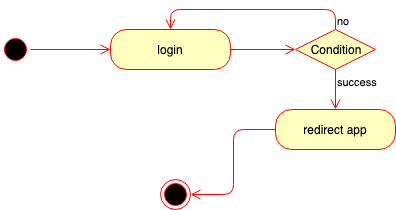
\includegraphics[width=0.5\textwidth]{./resources/act-dia-login}
		\caption{Diagram \textit{Activity} Untuk \textit{Login}}
		\label{fig:act-dia-login}
	\end{figure}
	
	Awalnya saat pengguna (\textit{resource owner}) mencoba melakukan akses yang membutuhkan \textit{login} dari aplikasi klien (\textit{user agent}), maka halaman \textit{login} akan muncul, kemudian pengguna mengisikan \textit{username} dan \textit{password} untuk melakukan otentikasi.
	
	Apabila kondisi otentikasi berhasil dilakukan, maka proses berikutnya pengguna akan diarahkan ke halaman data yang menjadi kewenangannya atau hak aksesnya (\textit{role}), namun bila gagal, pengguna akan tetap berada pada halaman \textit{login}.
	
	%2
	\item Diagram \textit{Activity} Menampilkan Daftar Pengguna (\textit{Resource Owner})

		Diagram \textit{activity} untuk menampilkan daftar pengguna yang telah terdaftar dalam sistem otentikasi adalah seperti berikut :
		
		\begin{figure}[H]
			\centering
			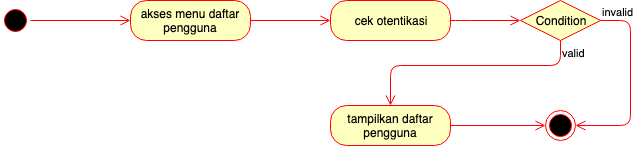
\includegraphics[width=1\textwidth]{./resources/act-dia-list-user}
			\caption{Diagram \textit{Activity} Untuk Menampilkan Daftar Pengguna (\textit{Resource Owner})}
			\label{fig:act-dia-list-user}
		\end{figure}
		
		Diagram tersebut menggambarkan pada saat akan melakukan akses ke menu untuk menampilkan daftar pengguna, prosesnya akan melalui pemeriksaan otentikasi, apakah pengguna (\textit{resource owner}) dalam kewenangannya melakukan akses terhadap halaman tersebut, bila ya, maka daftar pengguna akan ditampilkan, namun bila tidak, halaman tersebut tidak akan ditampilkan.
	
	%3
	\item Diagram \textit{Activity} Menambah Data Pengguna (\textit{Resource Owner})
	
	Diagram \textit{activity} untuk menambah data pengguna (\textit{resource owner}) baru pada sistem otentikasi adalah seperti berikut :
	
	\begin{figure}[H]
		\centering
		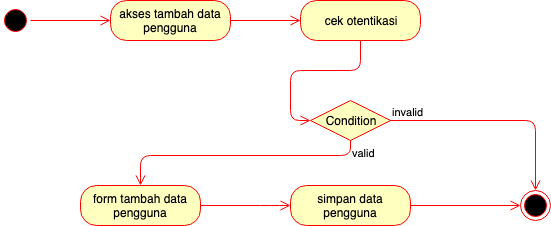
\includegraphics[width=1\textwidth]{./resources/act-dia-add-user}
		\caption{Diagram \textit{Activity} Untuk Menambah Data Pengguna (\textit{Resource Owner}) Baru}
		\label{fig:act-dia-add-user}
	\end{figure}	
	
	Diagram tersebut menjelaskan bahwa ketika ada akses ke fitur tambah data pengguna, maka akan dilakukan otentikasi terlebih dahulu, apabila hasil dari otentikasi menyatakan bahwa pengguna (\textit{resource owner}) tersebut memiliki hak akses (\textit{role}) atau kewenangan pada fitur ini, maka formulir tambah data akan ditampilkan kemudian dapat dilakukan simpan data padanya, namun bila otentikasi gagal, maka proses tidak akan menampilkan formulir tambah data pengguna.
	
	%4
	\item Diagram \textit{Activity} Mengubah Data Pengguna (\textit{Resource Owner})
	
		Diagram \textit{activity} untuk mengubah data pengguna (\textit{resource owner}) yang telah terrekam pada sistem otentikasi adalah seperti berikut ini :
		
		\begin{figure}[H]
			\centering
			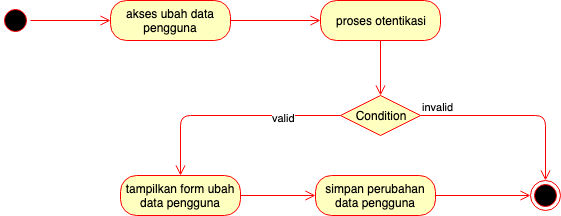
\includegraphics[width=1\textwidth]{./resources/act-dia-edit-user}
			\caption{Diagram \textit{Activity} Untuk Mengubah Data Pengguna (\textit{Resource Owner})}
			\label{fig:act-dia-edit-user}
		\end{figure}
		
		Diagram tersebut menjelaskan pada saat pengguna (\textit{resource owner}) melakukan akses ke fitur ubah data pengguna, maka proses otentikasi akan dijalankan, apabila pengguna (\textit{resource owner}) memiliki hak akses atau kewenangan untuk menggunakan fitur ini, maka formulir ubah data pengguna akan ditampilkan dan fitur untuk simpan hasil dari perubahan data pengguna dapat dilakukan, namun apabila otentikasi gagal, maka formulir tidak akan ditampilkan
	
	%5
	\item Diagram \textit{Activity} Menghapus Data Pengguna (\textit{Resource Owner})
	
	Diagram \textit{activity} untuk menghapus data pengguna (\textit{resource owner}) yang telah terrekam pada sistem otentikasi adalah seperti berikut :
	
	\begin{figure}[H]
		\centering
		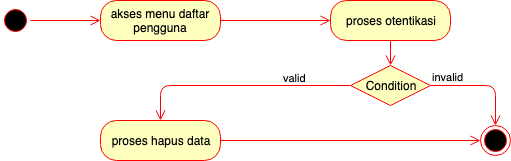
\includegraphics[width=1\textwidth]{./resources/act-dia-remove-user}
		\caption{Diagram \textit{Activity} Untuk Menghapus Data Pengguna (\textit{Resource Owner})}
		\label{fig:act-dia-remove-user}
	\end{figure}	
	
	Diagram tersebut menjelaskan pada saat pengguna akan melakukan proses hapus data pengguna (\textit{resource owner}), maka pengguna melakukan akses terhadap menu daftar pengguna terlebih dahulu, kemudian proses otentikasi akan terjadi, apabila pengguna (\textit{resource owner}) memiliki kewenangan akses terhadap fitur ini, maka pengguna dapat melakukan proses hapus data, apabila tidak memiliki kewenangan, maka fitur hapus data tidak dapat diakses oleh pengguna (\textit{resource owner}).
	
	%6
	\item Diagram \textit{Activity} Menampilkan Daftar Hak Akses (\textit{Role})
	
	Diagram \textit{activity} untuk menampilkan daftar hak akses / kewenangan (\textit{role}) yang telah terrekam pada sistem otentikasi adalah seperti berikut :
	
	\begin{figure}[H]
		\centering
		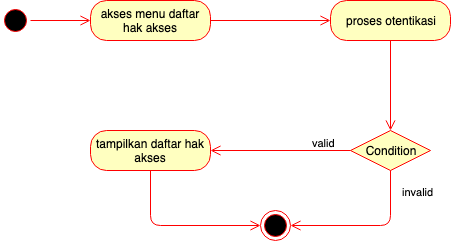
\includegraphics[width=1\textwidth]{./resources/act-dia-list-role}
		\caption{Diagram \textit{Activity} UntuK Menampilkan Hak Akses (\textit{Role})}
		\label{fig:act-dia-list-role}
	\end{figure}
	
	DIagram tersebut menjelaskan pada saat pengguna (\textit{resource owner}) akan melakukan akses terhadap daftar hak akses atau kewenangan (\textit{role}) yang kemudian akan dilakukan otentikasi terlebih dahulu apakah pengguna telah sesuai dengan kewenangannya melakukan akses terhadap daftar hak akses, apabila dinyatakan sesuai, maka aplikasi klien akan menampilkan daftar hak akses / kewenangan (\textit{role}), namun bisa tidak maka prosesnya akan dilewati.
	
	%7
	\item Diagram \textit{Activity} Menambahkan Hak Akses (\textit{Role})
	
	Diagram \textit{activity} untuk menambahkan data kewenangan (\textit{role}) dalam sistem otentikasi adalah seperti berikut :
	
	\begin{figure}[H]
		\centering
		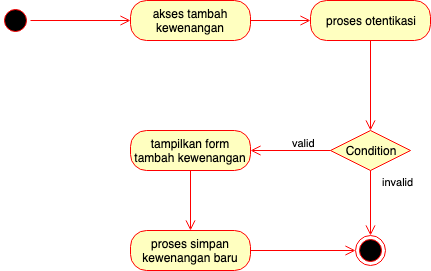
\includegraphics[width=1\textwidth]{./resources/act-dia-add-role}
		\caption{Diagram \textit{Activity} Untuk Menambahkan Data Kewenangan (\textit{Role})}
		\label{fig:act-dia-add-role}
	\end{figure}
	
	Diagram tersebut menjelaskan pada saat pengguna (\textit{resource owner}) akan melakukan akses ke fitur tambah kewenangan, maka proses otentikasinya berjalan untuk memastikan apakah pengguna (\textit{resource owner}) dalam kewenangannya untuk menambahkan data hak akses, bila ditemukan bahwa pengguna (\textit{resource owner}) memiliki kewenangan tersebut, maka formulir untuk menambahkan hak akses akan muncul dan proses simpan data kewenangan dapat dilakukan, setelah itu proses selesai, namun bila pengguna tidak memiliki kewenangan tersebut, maka prosesnya akan dilewati.
	
	%8
	\item Diagram \textit{Activity} Mengubah Hak Akses (\textit{Role})
	
	Diagram \textit{activity} untuk mengubah data kewenangan (\textit{role}) dalam sistem otentikasi adalah seperti berikut :
	
	\begin{figure}[H]
		\centering
		\includegraphics[width=1\textwidth]{./resources/act-dia-edit-role}
		\caption{Diagram \textit{Activity} Untuk Mengubah Data Kewenangan (\textit{Role})}
		\label{fig:act-dia-edit-role}
	\end{figure}	
	
	Diagram tersebut menjelaskan pada saat pengguna (\textit{resource owner}) akan melakukan akses ke ubah kewenangan, proses otentikasi akan dilakukan terhadap pengguna (\textit{resource owner}), bila pengguna (\textit{resource owner}) memiliki kewenangan untuk mengubah data, maka formulir untuk mengubah kewenangan (\textit{role}) akan ditampilkan, dan proses simpan perubahan data kewenangan dapat dialkukan, kemudian prosesnya selesai, namun bila pengguna (\textit{resource owner}) tidak memiliki hak atas perubahan tersebut, maka proses menampilkan form untuk mengubah data kewenangan dan proses simpan data akan dilewati.
	
	%9	
	\item Diagram \textit{Activity} Menghapus Hak Akses (\textit{Role})
	
	Diagram \textit{activity} untuk menghapus data kewenangan (\textit{role}) dalam sistem otentikasi adalah seperti berikut :
	
	\begin{figure}[H]
		\centering
		\includegraphics[width=1\textwidth]{./resources/act-dia-remove-role}
		\caption{Diagram \textit{Activity} Untuk Menghapus Data Kewenangan (\textit{Role})}
		\label{fig:act-dia-remove-role}
	\end{figure}
	
	Diagram tersebut menjelaskan pada saat pengguna (\textit{resource owner}) akan melakukan proses hapus data, pengguna (\textit{resource owner}) melakukan akses dulu ke tampilkan daftar kewenangan, setelah itu proses otentikasi akan berjalan untuk memastikan bahwa pengguna (\textit{resource owner}) dalam kewenangannya untuk melakukan hapus data kewenangan, bila pengguna (\textit{resource owner}) memiliki kewenangan (\textit{role}) untuk melakukan hapus data hak akses, maka fitur untuk menghapus data kewenangan dapat dilakukan, namun bila tidak prosesnya akan terlewati.
	
	%10
	\item Diagram \textit{Activity} Menampilkan Daftar Pemberian Hak Akses (\textit{Role})
	
	Diagram \textit{activity} untuk menampilkan daftar pemberian hak akses (\textit{role}) dalam sistem otentikasi akan terlihat seperti berikut :
	
	\begin{figure}[H]
		\centering
		\includegraphics[width=1\textwidth]{./resources/act-dia-list-user-role}
		\caption{Diagram \textit{Activity} Untuk Menampilkan Daftar Pemberian Hak Akses (\textit{Role})}
		\label{fig:act-dia-list-user-role}
	\end{figure}
	
	Diagram tersebut menjelaskan pada saat pengguna (\textit{resource owner}) melakukan akses untuk menampilkan daftar pemberian kewenangan, maka proses otentikasi akan terjadi, bila pengguna (\textit{resource owner}) memiliki kewenangan itu, maka daftar pemberian kewenangan akan ditampilkan, namun bila tidak, prosesnya akan dilewati.
	
	%11
	\item Diagram \textit{Activity} Menambahkan Pemberian Hak Akses (\textit{Role})
	
	Diagram \textit{activity} untuk menambahkan pemberian hak akses (\textit{role}) ke pengguna adalan seperti gambar berikut ini :
	
	\begin{figure}[H]
		\centering
		\includegraphics[width=1\textwidth]{./resources/act-dia-add-user-role}
		\caption{Diagram \textit{Activity} Untuk Menambahkan Pemberian Hak Akses (\textit{Role})}
		\label{fig:act-dia-add-user-role}
	\end{figure}	
	
	Diagram tersebut menjelaskan pada saat akan memberikan penambahan hak akses baru, pengguna (\textit{resource owner}) akan melakukan akses ke daftar pemberian hak akses terlebih dahulu, sampai sini proses otentikasi akan berjalan, bila pengguna (\textit{resource owner}) memiliki kewenangan itu, proses tambah hak akses (\textit{role}) akan dilakukan, namun bila tidak, maka prosesnya akan dilewati.
	
	%12
	\item Diagram \textit{Activity} Menghapus Pemberian Hak Akses (\textit{Role})
	
	Diagram \textit{activity} untuk menghapus pemberian hak akses (\textit{role}) yang telah tersimpan dalam sistem otentikasi adalah seperti gambar berikut :
	
	\begin{figure}[H]
		\centering
		\includegraphics[width=1\textwidth]{./resources/act-dia-remove-user-role}
		\caption{Diagram \textit{Activity} Untuk Menghapus Pemberian Hak Akses (\textit{Role})}
		\label{fig:act-dia-remove-user-role}
	\end{figure}
	
	Diagram tersebut menjelaskan pada saat pengguna (\textit{resource owner}) akan melakukan penghapusan terhadap pemberian kewenangan yang telah tersimpan dalam sistem otentikasi, pengguna (\textit{resource owner}) akan melakukan akses pada daftar pemberian hak akses (\textit{role}) terlebih dahulu, kemudian proses otentikasi akan berjalan, bila pengguna memiliki kewenangan untuk melakukan penghapusan pemberian kewenangan (\textit{role}) terhadap suatu pengguna (\textit{resource owner}), maka proses penghapusan dapat dilakukan, namun bila tidak, maka proses tersebut akan dilewati.
	
	%13
	\item Diagram \textit{Activity} Menampilkan Daftar Aplikasi Klien (\textit{User Agent})
	
	Diagram \textit{activity} untuk menampilkan daftar aplikasi klien (\textit{user agent}) yang telah terdaftar dalam sistem otentikasi ini adalah seperti pada gambar berikut :
	
	\begin{figure}[H]
		\centering
		\includegraphics[width=1\textwidth]{./resources/act-dia-list-client}
		\caption{Diagram \textit{Activity} Untuk Menampilkan Daftar Aplikasi Klien (\textit{User Agent})}
		\label{fig:act-dia-list-client}
	\end{figure}
	
	Diagram tersebut menjelaskan pada saat pengguna (\textit{resource owner}) akan melihat daftar aplikasi klien yang telah tersimpan dalam sistem otentikasi, aplikasi akan melalui proses otentikasi pengguna, apakah pengguna (\textit{resource owner}) dalam kapasitas atau kewenangannya memiliki hak untuk melihat daftar aplikasi klien (\textit{user agent}) atau tidak, bila ya (\textit{valid}), maka aplikasi akan menampilkan daftar aplikasi klien, namun bila tidak maka prosesnya akan dilewati.
	
	%14
	\item Diagram \textit{Activity} Menambah Data Aplikasi Klien (\textit{User Agent})
	
	Diagram \textit{activity} untuk menambah data aplikasi klien (\textit{user agent}) yang baru ke dalam sistem otentikasi adalah seperti gambar berikut :
	
	\begin{figure}[H]
		\centering
		\includegraphics[width=1\textwidth]{./resources/act-dia-add-client}
		\caption{Diagram \textit{Activity} Untuk Menambahkan Data Aplikasi Klien (\textit{User Agent})}
		\label{fig:act-dia-add-client}
	\end{figure}	
	
	Diagram tersebut menjelaskan pada saat pengguna melakukan akses ke fitur tambah data aplikasi klien (\textit{user agent}), proses otentikasi akan berjalan untuk memastikan bahwa pengguna (\textit{resource owner}) memiliki hak akses terhadap fitur ini, bila ya, maka aplikasi akan menampilkan formulir untuk mengisikan data dari aplikasi klien yang akan didaftarkan, kemudian proses simpan dapat dilakukan, namun bila proses otentikasi gagal dan menyatakan bahwa pengguna (\textit{resource owner}) tidak memiliki hak akses, maka prosesnya akan dilewati.	
	
	%15
	\item Diagram \textit{Activity} Mengubah Data Aplikasi Klien (\textit{User Agent})
	
	Diagram \textit{activity} untuk mengubah data aplikasi klien (\textit{user agent}) yang telah terrekam dalam sistem otentikasi adalah seperti pada gambar berikut :
	
	\begin{figure}[H]
		\centering
		\includegraphics[width=1\textwidth]{./resources/act-dia-edit-client}
		\caption{Diagram \textit{Activity} Untuk Mengubah Data Aplikasi Klien (\textit{User Agent})}
		\label{fig:act-dia-edit-client}
	\end{figure}
	
	Diagram tersebut akan menjelaskan proses simpan perubahan data dari aplikasi klien yang telah terrekam dalam sistem otentikasi, pertama pengguna (\textit{resource owner}) akan melakukan akses ke fitur perubahan data aplikasi klien, kemudian proses otentikasi akan berjalan dan memastikan apakah pengguna (\textit{resource owner}) memiliki hak akses untuk mengubah data aplikasi klien atau tidak, bila ya, maka aplikasi akan menampilkan formulir untuk menubah data aplikasi klien, kemudian proses simpan perubahan data aplikasi klien dapat dilakukan, namun bila pengguna (\textit{resource owner}) tidak memiliki hak akses, maka proses menampilkan formulir perubahan data aplikasi klien dan proses simpan data perubahan akan dilewati.
	
	%16
	\item Diagram \textit{Activity} Menghapus Data Aplikasi Klien (\textit{User Agent})
	
	Diagram \textit{activity} untuk menghapus data aplikasi klien (\textit{user agent}) yang telah terrekam dalam sistem otentikasi adalah seperti gambar berikut :
	
	\begin{figure}[H]
		\centering
		\includegraphics[width=1\textwidth]{./resources/act-dia-remove-client}
		\caption{Diagram \textit{Activity} Untuk Menghapus Data Aplikasi Klien (\textit{User Agent})}
		\label{fig:act-dia-remove-client}
	\end{figure}
	
	Diagram tersebut akan menjelaskan proses hapus data dari aplikasi klien yang terrekam dalam sistem otentikasi, pertama pengguna perlu melakukan akses ke tampilkan daftar aplikasi klien, setelah itu proses otentikasi akan berjalan untuk menentukan apakah pengguna memiliki kewenangan untuk menghapus data aplikasi klien yang telah terrekam atau tidak, bila ya, maka proses hapus data aplikasi klien dapat dilakukan, namun bila tidak, proses akan dilewatkan.
\end{itemize}

\subsubsection{Diagram \textit{Sequence}}

Diagram ini akan menggambarkan alur pertukaran pesan dari beberapa objek pada rentang siklus hidupnya. Diagram ini pun akan kita bagi menjadi beberapa bagian sesuai dengan \textit{case} atau fitur yang dimiliki oleh sistem otentikasi, berikut daftarnya :

\begin{itemize}
	%1
	\item Diagram \textit{Sequence Login}
	
	Diagram \textit{sequence} untuk proses \textit{login} akan digambarkan seperti berikut ini :
	
	\begin{figure}[H]
		\centering
		\includegraphics[width=1\textwidth]{./resources/seq-dia-login}
		\caption{Diagram \textit{Sequence} Untuk Proses \textit{Login}}
		\label{fig:seq-dia-login}
	\end{figure}
	
	Pertama pengguna (\textit{resource owner}) melakukan aksi untuk melakukan \textit{login} melalui \texttt{MainComponent}, \textit{method} yang dipanggil adalah \textit{method} \texttt{loginOAuth()}. 
	
	Selanjutnya dari \texttt{MainComponent} mengarahkan pengguna ke halaman \textit{login} pada \textit{OAuth Server}, setelah proses \textit{login} berhasil, \textit{OAuth Server} akan mengembalikan sebuah token ke \texttt{MainComponent} yang kemudian token ini disimpan pada \texttt{AuthService}.
	
	Tahap berikutnya \texttt{MainComponent} melakukan \textit{refresh} halaman untuk membuka beberapa menu sesuai dengan kewenangan pengguna yang sebelumnya disembunyikan.
	
	%2 
	\item Diagram \textit{Sequence} Untuk Menampilkan Daftar Pengguna (\textit{Resource Owner})
	
	Diagram \textit{sequence} untuk menampilkan daftar pengguna (\textit{resource owner}) adalah seperti gambar berikut :
	
	\begin{figure}[H]
		\centering
		\includegraphics[width=1\textwidth]{./resources/seq-list-user}
		\caption{Diagram \textit{Sequence} Untuk Menampilkan Daftar Pengguna}
		\label{fig:seq-list-user}
	\end{figure}
	
	Pertama pengguna (\textit{resource owner}) melakukan akses ke fitur menampilkan daftar pengguna melalui \texttt{MainUserComponent}. Kemudian aplikasi klien melakukan pemeriksaan kewenangan, apakah hak aksesnya memenuhi syarat atau tidak, apabila memenuhi syarat, maka akan ditampilkan daftar pengguna melalui \texttt{ListUserComponent}.
	
	Berikutnya \texttt{ListUserComponent} melakukan akses ke fungsi \texttt{getListUser()} milik \texttt{UserService}, yang kemudian diteruskan dalam bentuk \textit{request} ke \textit{resource server} oleh \texttt{UserService} melalui akses ke \textit{method} \texttt{getDaftarUser()} milik kelas \texttt{UserController}.
	
	\texttt{UserController} kemudian melakukan akses ke sistem basis data melalui \textit{method} \texttt{findAll()} milik \texttt{UsersRepo}. Hasil dari \textit{method} \texttt{findAll()} milik \texttt{UsersRepo} berupa \texttt{List<Users>} yang dikembalikan ke \texttt{UserController}.
	
	\texttt{UserController} kemudian mengirimkan \textit{response} ke aplikasi klien (\textit{user agent}) berupa \texttt{Flux<Users>} melalui \texttt{UserService} yang sebelumnya melakukan \textit{request}.
	
	Kemudian \texttt{UserService} meneruskan \textit{response} berupa \texttt{Observable} ke \texttt{ListUserComponent}, yang akhirnya digunakan untuk melakukan pembaruan data pada tabel yang dapat dikonsumsi oleh pengguna.
	
	%3 
	\item Diagram \textit{Sequence} Untuk Menambah Data Pengguna (\textit{Resource Owner})
	
		Diagram \textit{sequence} untuk proses menambahkan data pengguna (\textit{Resource Owner}) adalah seperti berikut :
		
		\begin{figure}[H]
			\centering
			\includegraphics[width=1\textwidth]{./resources/seq-add-user}
			\caption{Diagram \textit{Sequence} Untuk Menambahkan Data Pengguna}
			\label{fig:seq-add-user}
		\end{figure}
		
		Penjelasan dari diagram tersebut yaitu pertama, pengguna (\textit{resource owner}), dalam hal ini yang memiliki kewenangan tentu saja, melakukan akses ke formulir tambah data pengguna (\textit{resource owner}) melalui \texttt{AddUserComponent}, kemudian prosesnya berlanjut menampilkan \texttt{SearchUsernameProgressDialogComponent}, dari komponen ini melakukan akses ke fungsi \texttt{findUser()} milik \texttt{UserService}, dari \texttt{UserService} mencoba melakukan \textit{request} ke \textit{resource server}, dalam hal ini melalui \textit{method} \texttt{cariUser()} milik kelas \texttt{UserController}.
		
		\textit{Method} dari kelas \texttt{UserController} kemudian melakukan akses ke \textit{method} \texttt{getOne()} milik \texttt{UsersRepo}, yang kemudian akses ke sistem basis data terjadi. Apabila data yang dicari ada dalam sistem basis data, maka \textit{method} \texttt{getOne()} akan mengembalikan detail dari pengguna tersebut, namun bila tidak ditemukan, maka data yang dikembalikan adalah data kosong.
		
		Setelah \texttt{UserController} menerima \textit{response} atau data dari \texttt{UsersRepo}, \texttt{UserController} melakukan \textit{response} ke aplikasi klien, dalam hal ini melalui \texttt{UserService}, kemudian proses datanya berlanjut ke \texttt{SearchUsernameProgressDialogComponent} sampai kembali ke \texttt{AddUserComponent}.
		
		Bila data yang akan disimpan belum terdaftar dalam sistem basis data, maka dari \texttt{AddUserComponent} akan memanggil \texttt{SaveUserProgressComponent}, kemudian dari komponen \texttt{SaveUserProgressComponent} akan melakukan akses ke fungsi \texttt{saveUser()} milik \texttt{UserService}, yang kemudian dari fungsi tersebut akan berlanjut melakukan \textit{request} ke \textit{resource server} melalui \textit{method} \texttt{save} milik \texttt{UserController}.
		
		Dari \textit{method} \texttt{save} milik \texttt{UserController}, kemudian akan melakukan akses ke \textit{method} \texttt{save} milik \texttt{UsersService}, yang kemudian dari sini akan melakukan akses ke \textit{method} \texttt{saveAndFlush()} milik \texttt{UsersRepo}.
		
		Dari \textit{method} \texttt{saveAndFlush()} milik \texttt{UsersRepo} proses pencatatan ke sistem basis data terjadi, kemudian \textit{method} ini akan mengembalikan objek berupa \texttt{Users} ke \texttt{UsersService}, yang dilanjutkan dikirim ke \texttt{UserController}.
		
		Dari \texttt{UserController} kemudian akan melakukan \textit{response} ke aplikasi klien berupa objek \texttt{Users} dalam bentuk JSON, yang diterima di \texttt{UserService}.
		
		Dari \texttt{UserService} kemudian akan mengirimkan datanya ke \texttt{SaveUserProgressComponent} dalam bentuk \texttt{Observable} yang kemudian diteruskan pesannya dalam bentuk status ke \texttt{AddUserComponent}.
		
		Setelah \texttt{AddUserComponent} menangkap pesan dari \texttt{SaveUserProgressComponent}, kemudian memanggil \texttt{InfoDialogComponent} untuk memberitahu pengguna bahwa data yang diproses untuk disimpan telah tersimpan dalam sistem basis data.
	
	%4
	\item Diagram \textit{Sequence} Untuk Mengubah Data Pengguna (\textit{Resource Owner})
	
	Diagram \textit{sequence} untuk proses mengubah data pengguna (\textit{resource owner}) adalah seperti gambar berikut :
	
	\begin{figure}[H]
		\centering
		\includegraphics[width=1\textwidth]{./resources/seq-edit-user}
		\caption{Diagram \textit{Sequence} Untuk Mengubah Data Pengguna}
		\label{fig:seq-edit-user}
	\end{figure}	
	
	Penjelasan dari diagram tersebut adalah seperti berikut, pertama pengguna (\textit{resource owner}) melakukan akses ke fitur Ubah Data Pengguna pada daftar pengguna seperti ditunjukkan pada akses ke fungsi \texttt{onUbahClick()} milik \texttt{ListUserComponent}. Kemudian \texttt{ListUserComponent} melakukan pemanggilan ke \texttt{EditUserComponent} sehingga muncul jendela formulir untuk mengubah data pengguna (\textit{resource owner}).
	
	Setelah mengisi perubahan informasi data pengguna, maka pengguna (\textit{resource owner}) melakukan simpan perubahan data melalui fungsi \texttt{onSimpanClick()} milik \texttt{EditUserComponent}, kemudian komponen ini melakukan pemanggilan ke \texttt{SaveUserProgressComponent} untuk melanjutkan prosesnya menyimpan perubahan data pengguna.
	
	Kemudian \texttt{SaveUserProgressComponent} melakukan akses ke fungsi \texttt{saveUser()} milik \texttt{UserService} yang dilanjutkan dengan aksi \textit{request} dari \texttt{UserService} ke \textit{resource server}, dalam hal ini adalah \textit{method} \texttt{save()} milik \texttt{UserController}.
	
	Prosesnya kemudian berlanjut dari \texttt{UserController} melakukan akses ke \textit{method} \texttt{save()} milik \texttt{UsersService}, dan di dalamnya melakukan akses ke \textit{method} \texttt{saveAndFlush()} milik \texttt{UsersRepo}.
	
	Sampai sini proses interaksi dengan sistem basis data terjadi, setelah perubahan berhasil disimpan dalam sistem basis data, maka \texttt{UsersRepo} akan mengembalikan sebuah objek ke \texttt{UsersService} berbentuk kelas \texttt{Users} yang artinya data telah tersimpan.
	
	Objek \texttt{Users} akan diteruskan dari \texttt{UsersService} ke \texttt{UserController}, yang kemudian \texttt{UserController} akan memberikan \textit{response} ke aplikasi klien (\textit{user agent}), dalam hal ini ke \texttt{UserService} karena sebelumnya melakukan \textit{request}.
	
	Dari \texttt{UserService} kemudian akan mengembalikan data ke \texttt{SaveUserProgressComponent} dalam bentuk \texttt{Observable}, yang kemudian akan diteruskan ke \texttt{EditUserComponent}. Dari komponen \texttt{EditUserComponent} ini kemudian memanggil \texttt{InfoDialogComponent} untuk memberitahukan status berhasil atau tidaknya hasil perubahan disimpan dalam sistem basis data ke pengguna (\texttt{resource owner}).
	
	Terakhir dari \texttt{InfoDialogComponent} kemudian akan mengembalikan halaman aktif ke \texttt{ListUserComponent} yang kemudian akan melakukan pembaruan data pada tabel agar data yang telah diubah diketahui perubahannya.
	
	%5
	\item Diagram \textit{Sequence} Untuk Menghapus Data Pengguna (\textit{Resource Owner})
	
	Diagram \textit{sequence} untuk proses penghapusan data pengguna (\textit{resource owner)} dari sistem otentikasi adalah seperti gambar berikut :
	
	\begin{figure}[H]
		\centering
		\includegraphics[width=1\textwidth]{./resources/seq-del-user}
		\caption{Diagram \textit{Sequence} Untuk Menghapus Data Pengguna}
		\label{fig:seq-del-user}
	\end{figure}
	
	Penjelasan dari diagram tersebut adalah seperti berikut, pertama pengguna (\textit{resource server}) menggunakan fitur hapus data pengguna melalui fungsi \texttt{onHapusClick()} milik \texttt{ListUserComponent}, kemudian \texttt{ListUserComponent} melakukan pemanggilan ke \texttt{KonfirmasiDialogComponent} untuk melakukan konfirmasi apakah pengguna (\textit{resource owner}) akan menghapus data tersebut.
	
	Bila pengguna (\textit{resource owner}) melakukan konfirmasi untuk hapus data, prosesnya akan berlanjut ke pemanggilan \texttt{RemoveUserProgressDialogComponent}, yang di dalamnya akan memanggil fungsi \texttt{removeUser()} milik \texttt{UserService}.
	
	Selanjutnya \texttt{UserService} melakukan \textit{request} ke \textit{resource server} melalui \textit{method} \texttt{removeUser()} milik \texttt{UserController}. Setelah itu \texttt{UserController} akan melakukan akses ke \textit{method} \texttt{deleteById()} milik \texttt{UsersRepo} yang kemudian melakukan operasi hapus data pada sistem basis data.
	
	Kemudian \textit{method} \texttt{deleteById()} mengembalikan sebuah nilai ke \texttt{UserController} dan diteruskan menjadi \textit{response} ke aplikasi klien, dalam hal ini melalui \texttt{UserService} yang sebelumnya melakukan \textit{request}.
	
	Hasil \textit{response} ini kemudian diteruskan ke \texttt{RemoveUserProgressDialogComponent} dalam bentuk \texttt{Observable}, yang kemudian dilanjutkan ke \texttt{ListUserComponent} dalam bentuk status. Dari status tersebut kemudian \texttt{ListUserComponent} melakukan pemanggilan ke \texttt{InfoDialogComponent} untuk memberitahu pengguna (\textit{resource owner}) apakah datanya telah terhapus atau belum yang kemudian aplikasi klien akan melakukan pembaruan data pada tabelnya.
	
	%6
	\item Diagram \textit{Sequence} Untuk Menampilkan Daftar Hak Akses (\textit{Role})
	
	Diagram \textit{sequence} untuk menampilkan daftar hak akses (\textit{role}) yang telah terrekam dalam sistem otentikasi adalah seperti gambar berikut :
	
	\begin{figure}[H]
		\centering
		\includegraphics[width=1\textwidth]{./resources/seq-list-role}
		\caption{Diagram \textit{Sequence} Untuk Menampilkan Daftar Hak Akses}
		\label{fig:seq-list-role}
	\end{figure}	
	
	Penjelasan dari diagram tersebut adalah seperti berikut, pertama pengguna (\textit{resource owner}) melakukan akses ke fitur menampilkan hak akses melalui fungsi \texttt{listHakAkses()} milik \texttt{MainUserComponent}, pada proses ini, fungsi \texttt{canActivate()} milik \texttt{CekLoginGuard} akan terpicu untuk melakukan verifikasi hak akses pengguna apakah memiliki kewenangan (\textit{role}) tersebut atau tidak.
	
	Bila pengguna memang memiliki hak akses, maka halaman akan diarahkan ke \texttt{ListRoleComponent} tempat daftar hak akses akan ditampilkan, di awalnya \texttt{ListRoleComponent} akan melakukan akses ke fungsi \texttt{getAllRole()} milik \texttt{RoleService}, kemudian \texttt{RoleService} melakukan \textit{request} ke \textit{resource server} melalui \textit{method} \texttt{getAllRoles()} milik \texttt{RoleController}.
	
	Kemudian \texttt{RoleController} akan melakukan akses ke \textit{method} \texttt{getAllData()} milik \texttt{RolesService}, yang kemudian dari \texttt{RolesService} melakukan akses ke \textit{method} \texttt{findAll()} milik \texttt{RolesRepo}. Dari \texttt{RolesRepo} inilah akses data ke sistem basis data terjadi yang kemudian akan mengembalikan nilai ke \texttt{RolesService} dalam bentuk \texttt{List<Roles>}.
	
	Dari \texttt{RolesService} kemudian mengembalikan nilai ke \texttt{RoleController} dalam bentuk \texttt{Flux<Roles>}, yang kemudian digunakan sebagai bahan \textit{response} ke aplikasi klien yang sebelumnya melakukan \textit{request}, data akan diterima di aplikasi klien melalui \texttt{RoleService}.
	
	Hasil yang diterima \texttt{RoleService} akan diteruskan ke \texttt{ListRoleComponent} dalam bentuk \texttt{Observable} yang kemudian digunakan sebagai bahan untuk melakukan pembaruan isi tabel daftar hak akses.
	
	%7
	\item Diagram \textit{Sequence} Untuk Menambahkan Hak Akses (\textit{Role})
	
	Diagram \textit{sequence} untuk menambahkan data hak akses (\textit{role}) adalah seperti pada gambar berikut :
	
	\begin{figure}[H]
		\centering
		\includegraphics[width=1\textwidth]{./resources/seq-add-role}
		\caption{Diagram \textit{Sequence} Untuk Menambahkan Data Hak Akses}
		\label{fig:seq-add-role}
	\end{figure}	
	
	Penjelasan dari diagram tersebut adalah seperti berikut, pertama pengguna melakukan akses ke fitur \texttt{ListRoleComponent}, kemudian melakukan akses ke fungsi \texttt{onAddRoleClick()} milik \texttt{ListRoleComponent}. Dari \texttt{ListRoleComponent} kemudian memanggil \texttt{AddRoleComponent} yang ditampilkan kepada pengguna untuk kemudian mengisikan data mengenai hak akses yang akan dibuatkan.
	
	Setelah pengguna (\textit{resource owner}) mengisikan data hak akses (\textit{role}), pengguna akan menekan tombol simpan yang akan memicu akses ke fungsi \texttt{onSaveClick()} milik \texttt{AddRoleComponent}. Dari dalam fungsi \texttt{onSaveClick()} ini akan memanggil \texttt{SearchRoleProgressDialog} melalui fungsi \texttt{ngOnInit()}, kemudian dari fungsi \texttt{ngOnInit()} milik \texttt{SearchRoleProgressDialog} melakukan akses ke fungsi \texttt{findById()} ke \texttt{RoleService}.
	
	Pada tahap ini, \texttt{RoleService} melakukan \textit{request} ke \textit{resource server} melalui \textit{method} \texttt{findById()} milik kelas \texttt{RoleController}, kemudian di dalamnya akan melakukan akses ke \textit{method} \texttt{findById()} milik \texttt{RolesService}, yang di dalamnya akan melakukan akses ke \textit{method} \texttt{findById()} milik \texttt{RolesRepo}.
	
	Pada operasi di \textit{method} \texttt{findById()} milik \texttt{RolesRepo} akan terjadi proses pencarian data pada sistem basis data, yang kemudian akan memberikan sebuah nilai balik berupa objek dari kelas \texttt{Optional<Roles>}, nilai ini dikirimkan ke \texttt{RolesService}.
	
	Dari \texttt{RolesService}, objek dari \texttt{Optional<Roles>} akan dikirimkan ke \texttt{RoleController}. Kemudian \texttt{RoleController} akan mengirimkan objek tersebut sebagai \textit{response} ke aplikasi klien melalui \texttt{RoleService} yang sebelumnya telah melakukan \textit{request}.
	
	Dari \texttt{RoleService} kemudian data hasil \textit{response} \textit{resource server} akan diteruskan ke \texttt{SearchRoleProgressDialog} dalam bentuk \texttt{Observable} yang kemudian diteruskan ke \texttt{AddRoleComponent}. Di \texttt{AddRoleComponent} kemudian akan melakukan seleksi apakah data hak akses sudah pernah dibuat atau belum, bila belum, maka proses berikutnya adalah memanggil \texttt{SaveRoleProgressDialogComponent} untuk melakukan simpan data.
	
	Di awal pemanggilan \texttt{SaveRoleProgressDialogComponent} akan melakukan pemanggilan ke fungsi \texttt{saveRole()} milik \texttt{RoleService}, yang kemudian diteruskan menjadi \textit{request} ke \textit{resource server} melalui \textit{method} \texttt{save()} milik \texttt{RoleController}.
	
	Dari \texttt{RoleController} kemudian melakukan akses ke \textit{method} \texttt{save()} milik \texttt{RolesService}, yang di dalamnya melakukan akses ke \textit{method} \texttt{saveAndFlush()}, disini akses simpan data terjadi pada sistem basis data.
	
	Setelah operasi simpan data pada sistem basis data selesai, \texttt{RolesRepo} mengembalikan sebuah nilai berupa objek \texttt{Roles} ke \texttt{RolesService}, yang kemudian diteruskan oleh \texttt{RolesService} ke \texttt{RoleController}.
	
	Setelah itu \texttt{RoleController} akan mengirimkan sebuah \textit{response} ke aplikasi klien melalui \texttt{RoleService} karena sebelumnya melakukan \textit{request} simpan data. Dari \texttt{RoleService} datanya diteruskan ke \texttt{SaveRoleProgressDialogComponent} dalam bentuk \texttt{Observable}, yang kemudian diolah dan mengirimkan status ke \texttt{AddRoleComponent}, dari status ini kemudian \texttt{AddRoleComponent} melakukan pemanggilan ke \texttt{InfoDialogComponent}, yang kemudian akan melakukan pengalihan tampilan ke \texttt{ListRoleComponent} yang secara otomatis akan melakukan pembaruan isi tabel daftar hak akses.
	
	%8
	\item Diagram \textit{Sequence} Untuk Mengubah Hak Akses (\textit{Role})
	
	Diagram \textit{sequence} untuk mengubah data hak akses (\textit{role}) adalah seperti pada gambar berikut :
	
	\begin{figure}[H]
		\centering
		\includegraphics[width=1\textwidth]{./resources/seq-edit-role}
		\caption{Diagram \textit{Sequence} Untuk Mengubah Data Hak Akses}
		\label{fig:seq-edit-role}
	\end{figure}
	
	Penjelasan dari diagram tersebut adalah seperti berikut, pertama pengguna melakukan akses ke fitur ubah data melalui fungsi \texttt{onEditRoleClick()} milik \texttt{ListRoleComponent}, kemudian \texttt{EditRoleComponent} akan dipanggil dan pengguna dapat mengisikan perubahan data pada komponen ini.
	
	Selanjut pada saat pengguna (\textit{user agent}) melakukan simpan data perubahan, prosesnya akan mengakses fungsi \texttt{onSaveClick()} milik \texttt{EditRoleComponent}, di dalam fungsi \texttt{onSaveClick()} ini kemudian akan memanggil \texttt{SaveRoleProgressDialogComponent} untuk memulai proses simpan data perubahannya.
	
	Di dalam \texttt{SaveRoleProgressDialogComponent} akan melakukan akses ke fungsi \texttt{saveRole()} milik \texttt{RoleService}, yang kemudian dari \texttt{RoleService} akan melakukan \textit{request} ke \textit{resource server} melalui \textit{method} \texttt{save} milik kelas \texttt{RoleController}.
	
	Dari kelas \texttt{RoleController}, kemudian akan melakukan akses ke \textit{method} \texttt{save()} milik \texttt{RolesService}, yang diteruskan di dalam \texttt{RolesService} untuk melakukan akses ke \textit{method} \texttt{saveAndFlush()} milik \texttt{RolesRepo}. Pada tahap inilah proses simpan data ke sistem basis data terjadi.
	
	Setelah proses simpan data ke sistem basis data berhasil, \texttt{RolesRepo} akan mengembalikan sebuah objek dalam bentuk \texttt{Roles} ke \texttt{RolesService}, yang kemudian dari \texttt{RolesService} akan diteruskan ke \texttt{RoleController}.
	
	Nilai dari objek \texttt{Roles} kemudian dijadikan bahan \textit{response} data ke aplikasi klien melalui \texttt{RoleService} karena sebelumnya melakukan \textit{request}. Dari \textit{RoleService} kemudian hasil \textit{response} akan dikirimkan ke \texttt{SaveRoleProgressDialogComponent} dalam bentuk \texttt{Observable}, yang kemudian diteruskan ke \texttt{EditRoleComponent} dalam bentuk status.
	
	Nilai kembalian dalam bentuk status ini akan menjadi pemicu untuk kemudian memanggil \texttt{InfoDialogComponent} untuk memberikan informasi ke pengguna (\textit{resource owner}) apakah data perubahan berhasil tersimpan atau tidak ke sistem basis data, yang pada akhirnya akan menjadi pemicu untuk melakukan pembaruan data tabel pada \texttt{ListRoleComponent}.
	
	%9 
	\item Diagram \textit{Sequence} Untuk Menghapus Hak Akses (\textit{Role})
	
	Diagram \textit{sequence} untuk menghapus hak akses (\textit{role}) adalah seperti pada gambar berikut :
	
	\begin{figure}[H]
		\centering
		\includegraphics[width=1\textwidth]{./resources/seq-del-role}
		\label{fig:seq-del-role}
		\caption{Diagram \textit{Sequence} Untuk Menghapus Data Hak Akses}
	\end{figure}
	
	Penjelasan dari diagram tersebut adalah seperti berikut ini, pertama pengguna berada pada \texttt{ListRoleComponent} dan memilih salah satu data untuk dihapus melalui fungsi \texttt{onRemoveRoleClick()} milik \texttt{ListRoleComponent}. Dari dalam fungsi ini kemudian memanggil \texttt{KonfirmasiDialogComponent} untuk memastikan bahwa data yang terpilih untuk dihapus adalah benar.
	
	Setelah pengguna (\textit{user agent}) memastikan data tersebut akan dihapus, kemudian prosesnya berlanjut dengan memanggil \texttt{RemoveRoleProgressDialogComponent}, yang di dalamnya akan menggunakan fungsi \texttt{removeRole()} milik \texttt{RoleService}.
	
	Di dalam fungsi \texttt{removeRole()} milik \texttt{RolesService}, prosesnya akan melakukan \textit{request} ke \textit{resource server} melalui \textit{method} \texttt{remove()} milik \texttt{RoleController}. Kemudian dari \texttt{RoleController} akan melakukan akses ke \textit{method} \texttt{remove()} milik \texttt{RolesService}, dan di dalam \textit{method} ini akan melakukan akses ke \textit{method} \texttt{deleteById()} milik \texttt{RolesRepo}.
	
	Di \texttt{RolesRepo} proses interaksi dengan sistem basis data terjadi, data pada sistem basis data akan dihapus dan proses berikutnya akan mengembalikan nilai ke \texttt{RolesService} yang kemudian diteruskan dari \texttt{RolesService} ke \texttt{RoleController}.
	
	Nilai kembalian yang diterima di \texttt{RoleController} digunakan sebagai bahan \textit{response} ke aplikasi klien yang kemudian diterima di \texttt{RoleService} karena sebelumnya melakukan \textit{request}. Setelah itu dari \texttt{RoleService} kemudian meneruskan hasilnya ke \texttt{RemoveRoleProgressDialogComponent} dalam bentuk \texttt{Observable}.
	
	Hasil yang diterima \texttt{RemoveRoleProgressDialogComponent} akan diteruskan dalam bentuk status ke \texttt{ListRoleComponent}, yang dengan nilai status ini kemudian \texttt{ListRoleComponent} melakukan pembaruan data pada tabel.
	
	%10
	\item Diagram \textit{Sequence} Untuk Menampilkan Daftar Pemberian Hak Akses (\textit{Role})
	
	Diagram \textit{sequence} untuk menampilkan pemberian hak akses adalah seperti pada gambar berikut :
	
	\begin{figure}[H]
		\centering
		\includegraphics[width=1\textwidth]{./resources/seq-list-user-role}
		\caption{Diagram \textit{Sequence} Untuk Menampilkan Daftar Pemberian Hak Akses}
		\label{fig:seq-list-user-role}
	\end{figure}
	
	Penjelasan dari diagram tersebut adalah sebagai berikut, pertama pengguna melakukan akses dari \texttt{MainUserComponent} ke menu Pemberian Hak Akses, menu ini akan melakukan akses ke fungsi \texttt{assignRoleClick()} yang di dalamnya akan memicu pemanggilan fungsi \texttt{canActivate()} milik \texttt{CekLoginGuard}, untuk memastikan bahwa pengguna (\textit{resource owner}) memiliki kewenangan untuk melakukan akses ke fitur tersebut.
	
	Setelah pengguna dinyatakan berhak atas akses tersebut, maka halaman akan dialihkan ke \texttt{AssignUserRoleComponent} yang di dalamnya akan melakukan akses ke fungsi \texttt{getAllUserRole()} milik \texttt{UserRoleService}.
	
	Dari dalam fungsi \texttt{getAllUserRole()} kelas \texttt{UserRoleService} melakukan \textit{request} ke \textit{resource server} melalui \textit{method} \texttt{getAllUserRole()} milik kelas \texttt{UserRoleController}, yang kemudian di dalam \textit{method} \texttt{getAllUserRole()} ditindak lanjuti dengan akses ke \textit{method} \texttt{getAllUserRole()} milik \texttt{UserRoleService}, yang di dalamnya melakukan akses ke \textit{method} \texttt{findAll()} milik \texttt{UserRoleRepo}. Pada tahap ini akses ke sistem basis data terjadi untuk mengambil daftar pemberian hak akses yang tercatat.
	
	Hasil dari pengambilan data pada sistem basis data oleh \texttt{UserRoleRepo} akan mengembalikan nilai berupa \texttt{List<UserRole>} ke \texttt{UserRoleService} yang kemudian diteruskan ke \texttt{UserRoleController} dalam bentuk \texttt{Flux<UserRole>}.
	
	Pada tahap ini \texttt{UserRoleController} akan mengirimkan sebuah \textit{response} ke aplikasi klien berupa objek \texttt{Flux<UserRole>} yang kemudian diterima oleh \texttt{UserRoleService} yang sebelumnya melakukan \textit{request}.
	
	Hasil \textit{response} dari \textit{resource server} kemudian dikirimkan oleh \texttt{UserRoleService} ke \texttt{AssignUserRoleComponent} dalam bentuk \texttt{Observable} yang kemudian digunakan untuk mengisi tabel daftar pemberian hak akses.
	
	%11
	\item Diagram \textit{Sequence} Untuk Menambahkan Pemberian Hak Akses (\textit{Role})
	
	Diagram \textit{sequence} untuk menambah pemberian hak akses adalah seperti pada gambar berikut :
	
	\begin{figure}[H]
		\centering
		\includegraphics[width=1\textwidth]{./resources/seq-add-user-role}
		\caption{Diagram \textit{Sequence} Untuk Menambah Pemberian Hak Akses}
		\label{fig:seq-add-user-role}
	\end{figure}
	
	Penjelasan dari diagram tersebut adalah seperti berikut, pertama pengguna melakukan proses simpan data melalui fungsi \texttt{onSimpanClick()} milik \texttt{AssignUserRoleComponent}, yang di dalamnya kemudian memanggil \texttt{SaveUserRoleProgressDialogComponent}. 
	
	Proses inisiasi yang terjadi pada \texttt{SaveUserRoleProgressDialogComponent} ketika dipanggil akan melakukan akses ke fungsi \texttt{save} milik \texttt{UserRoleService}, yang kemudian dari fungsi \texttt{save} ini, \texttt{UserRoleService} melakukan \textit{request} ke \textit{resource server} melalui \textit{method} \texttt{save} milik \texttt{UserRoleController}.
	
	Di dalam \textit{method} \texttt{save} milik \texttt{UserRoleController} kemudian melakukan akses ke \textit{method} \texttt{save} milik \texttt{UserRoleService}, yang di dalam \textit{method} ini akan melakukan akses ke \textit{method} \texttt{save} milik \texttt{UserRoleRepo}. Sampai sini proses interaksi dengan sistem basis data terjadi, data yang disertakan akan tersimpan dalam sistem basis data.
	
	Setelah proses simpan data berhasil tercatat dalam sistem basis data, \texttt{UserRoleRepo} akan mengembalikan nilai dalam bentuk objek \texttt{UserRole} ke \texttt{UserRoleService} yang kemudian hasilnya diteruskan ke \texttt{UserRoleController}.
	
	Setelah \texttt{UserRoleController} menerima data dari \texttt{UserRoleService}, \texttt{UserRoleController} akan mengirimkan \textit{response} ke aplikasi klien, dalam hal ini ke \texttt{UserRoleService} karena sebelumnya melakukan \textit{request} simpan data.
	
	Dari \texttt{UserRoleService} kemudian hasil \textit{response} akan diteruskan ke \texttt{SaveUserRoleProgressDialogComponent} dalam bentuk \texttt{Observable} yang kemudian dari \texttt{SaveUserRoleProgressDialogComponent} akan diteruskan ke \texttt{AssignUserRoleComponent} untuk melakukan pembaruan data pada tabel.
	
	%12
	\item Diagram \textit{Sequence} Untuk Menghapus Pemberian Hak Akses (\textit{Role})
	
	Diagram \textit{sequence} untuk menghapus pemberian hak akses adalah seperti pada gambar berikut ini :
	
	\begin{figure}[H]
		\centering
		\includegraphics[width=1\textwidth]{./resources/seq-del-user-role}
		\caption{Diagram \textit{Sequence} Untuk Menghapus Pemberian Hak Akses}
		\label{fig:seq-del-user-role}
	\end{figure}
	
	Penjelasan untuk diagram tersebut adalah seperti berikut, pertama pengguna (\textit{resource owner}) melakukan akses ke hapus data melalui fungsi \texttt{onHapusClick()} milik \texttt{AssignUserRoleComponent}, di dalamnya akan memanggil \texttt{RemoveUserRoleProgressDialogComponent} untuk memulai proses hapus data pemberian hak akses.
	
	Pada saat inisiasi \texttt{RemoveUserRoleProgressDialogComponent}, di dalamnya akan melakukan akses ke fungsi \texttt{remove} milik \texttt{UserRoleService}, dari dalam fungsi \texttt{remove} milik \texttt{UserRoleService} kemudian melakukan \textit{request} ke \textit{resource server} melalui \textit{method} \texttt{remove()} milik \texttt{UserRoleController}. 
	
	Lebih dalam, pada \textit{method} \texttt{remove()} milik \texttt{UserRoleController} akan melakukan akses ke \textit{method} \texttt{remove()} milik \texttt{UserRoleService}, lebih ke dalam lagi, dari \texttt{UserRoleService} akan melakukan akses ke \textit{method} \texttt{remove} milik \texttt{UserRoleRepo}. Di sini interaksi dengan sistem basis data terjadi, data akan dihapuskan dari sistem basis data.
	
	Proses selanjutnya \texttt{UserRoleRepo} akan mengembalikan sebuah nilai dalam bentuk objek \texttt{Unit} yang sebetulnya nilai kosong ke \texttt{UserRoleService}, yang kemudian diteruskan ke \texttt{UserRoleController}.
	
	Kemudian \texttt{UserRoleController} akan memberikan \texttt{response} ke aplikasi klien, melalui \texttt{UserRoleService} karena sebelumnya melakukan \textit{request}. Dari \texttt{UserRoleService}, data akan diteruskan ke \texttt{RemoveUserRoleProgressDialogComponent} dalam bentuk \texttt{Observable}, yang kemudian diolah dan diteruskan ke \texttt{AssignUserRoleComponent} dalam bentuk status, yang pada akhirnya statusnya digunakan untuk memicu pembaruan data pada tabel.
	
	%13
	\item DIagram \textit{Sequence} Untuk Menampilkan Daftar Aplikasi Klien (\textit{User Agent})
	
	Diagram \textit{sequence} untuk menampilkan daftar aplikasi klien adalah seperti pada gambar berikut :
	
	\begin{figure}[H]
		\centering
		\includegraphics[width=1\textwidth]{./resources/seq-list-client}
		\caption{Diagram \textit{Sequence} Untuk Menampilkan Daftar Aplikasi Klien}
		\label{fig:seq-list-client}
	\end{figure}
	
	Penjelasan dari diagram tersebut adalah seperti berikut, pertama pengguna (\textit{resource owner}) melakukan akses ke fitur Daftar Aplikasi Klien dengan cara melakukan akses melalui fungsi \texttt{onKlienClick()} milik \texttt{MainUserComponent}, yang kemudian akan memicu fungsi \texttt{canActivate()} milik \texttt{CekLoginGuard} tereksekusi untuk memeriksa apakah pengguna yang sedang melakukan akses berada dalam kewenangannya untuk melakukan hal tersebut.
	
	Bila kewenangannya memang memiliki hak akses untuk fitur tersebut, maka proses berikutnya adalah memanggil \texttt{ListOauthClientComponent}, yang pada tahap inisiasinya akan melakukan akses ke fungsi \texttt{getAllClient()} milik \texttt{OauthClientService}.
	
	Dari \texttt{OauthClientService} kemudian melakukan \texttt{request} ke \textit{resource server} melalui \textit{method} \texttt{getAllClient()} milik \texttt{OauthClientController}. Dari \texttt{OauthClientController} kemudian melakukan akses ke \textit{method} \texttt{getAllClient()} milik \texttt{OauthClientDetailsService}, selanjutnya \texttt{OauthClientDetailsService} melakukan akses ke \textit{method} \texttt{findAll()} milik \texttt{OauthClientDetailsRepo}. Sampai sini proses pengambilan seluruh data aplikasi klien terjadi pada lapisan sistem basis data.
	
	Setelah pengambilan data dari sistem basis data berhasil, kemudian nilai akan dikembalikan dari \texttt{OauthClientDetailsRepo} ke \texttt{OauthClientDetailsService} dalam bentuk objek \texttt{List<OauthClientDetails>}, yang kemudian diteruskan oleh \texttt{OauthClientDetailsService} ke \texttt{OauthClientController}.
	
	Dari \texttt{OauthClientController} kemudian melakukan \textit{response} ke aplikasi klien melalui \texttt{OauthClientService} karena sebelumnya melakukan \textit{request}, nilai yang diberikan ke aplikasi klien berbentuk objek \texttt{Flux<OauthClientDetails>}.
	
	Dari \texttt{OauthClientService}, hasil \textit{response} diteruskan ke \texttt{ListOauthClientComponent} dalam bentuk \texttt{Observable} yang kemudian menjadi bahan data untuk mengisikan tabel daftar aplikasi klien.
	
	%14
	\item Diagram \textit{Sequence} Untuk Menambahkan Data Aplikasi Klien (\textit{User Agent})
	
	Diagram \textit{sequence} untuk menambahkan data aplikasi klien adalah seperti pada gambar berikut :
	
	\begin{figure}[H]
		\centering
		\includegraphics[width=1\textwidth]{./resources/seq-add-client}
		\caption{Diagram \textit{Sequence} Untuk Menambahkan Daftar Aplikasi Klien}
		\label{fig:seq-add-client}
	\end{figure}
	
	Penjelasan dari diagram tersebut adalah seperti berikut, pertama pengguna (\textit{resource owner}) melakukan akses ke fitur tambah aplikasi klien melalui fungsi \texttt{onTambahKlienClick()} milik \texttt{ListOauthClientComponent}. Dari fungsi ini kemudian melakukan panggilan ke \texttt{AddOauthClientComponent} sehingga pengguna (\textit{resource owner}) dapat melakukan pengisian data aplikasi klien.
	
	Setelah pengguna (\textit{resource owner}) melakukan pengisian data aplikasi klien kemudian menyimpannya, maka fungsi \texttt{onSimpanClick()} pada \texttt{AddOauthClientComponent} akan terpicu, kemudian memanggil \texttt{CheckOauthClientProgressDialogComponent} untuk melakukan pemeriksaan data apakah aplikasi klien yang akan disimpan sudah pernah disimpan sebelumnya.
	
	Dari \texttt{CheckOauthClientProgressDialogComponent} kemudian melakukan akses ke fungsi \texttt{findById()} milik \texttt{OauthClientService}. Dari \texttt{OauthClientService} kemudian melakukan \textit{request} ke \textit{resource server} melalui \textit{method} \texttt{getById()} milik \texttt{OauthClientController}.
	
	Dari \texttt{OauthClientController} kemudian melakukan akses ke \textit{method} \texttt{findById()} milik \texttt{OauthClientDetailsService} yang di dalamnya melakukan akses ke \textit{method} \texttt{findById()} milik \texttt{OauthClientDetailsRepo}. Di sini proses pencarian data pada sistem basis data terjadi.
	
	Setelah proses pencarian data pada sistem basis data selesai, maka \texttt{OauthClientDetailsRepo} akan mengembalikan nilai dalam bentuk objek \texttt{Optional<OauthClientDetails>} ke \texttt{OauthClientDetailsService}, yang nilainya kemudian diteruskan ke \texttt{OauthClientController}.
	
	Kemudian \texttt{OauthClientController} akan melakukan \textit{response} ke aplikasi klien melalui \texttt{OauthClientService} karena sebelumnya melakukan \textit{request}. Dari \texttt{OauthClientService} kemudian hasil \textit{response} diteruskan ke \texttt{CheckOauthClientProgressDialogComponent} dalam bentuk \texttt{Observable} dan diteruskan ke \texttt{AddOauthClientComponent} dalam bentuk status.
	
	Bila status menunjukkan data yang akan disimpan belum pernah tercatat dalam sistem basis data, maka proses akan berlanjut dengan memanggil \texttt{SaveOauthClientProgressDialogComponent}, yang di dalamnya akan melakukan akses ke fungsi \texttt{save()} milik \texttt{OauthClientService}. Dari \texttt{OauthClientService} kemudian melakukan \textit{request} kembali ke \textit{resource server}, kali ini melalui \textit{method} \texttt{save()} milik \texttt{OauthClientController}.
	
	Dari \texttt{OauthClientController} kemudian melakukan akses ke \textit{method} \texttt{save()} milik \texttt{OauthClientDetailsService} yang di dalamnya melakukan akses ke \textit{method} \texttt{save()} milik \texttt{OauthClientDetailsRepo}. Sampai sini proses simpan data ke sistem basis data terjadi.
	
	Setelah data tersimpan pada sistem basis data, \texttt{OauthClientDetailsRepo} akan mengembalikan nilai dalam bentuk objek \texttt{OauthClientDetails} ke \texttt{OauthClientDetailsService}, yang kemudian diteruskan ke \texttt{OauthClientController}.
	
	Sampai tahap ini \texttt{OauthClientController} akan memberikan \textit{response} ke aplikasi klien melalui \texttt{OauthClientService} karena sebelumnya melakukan \textit{request}. Dari \texttt{OauthClientService}, \textit{response} akan diteruskan ke \texttt{SaveOauthClientProgressDialogComponent} dalam bentuk \texttt{Observable}. Dari \texttt{SaveOauthClientProgressDialogComponent} meneruskan pesan ini dalam bentuk status ke \texttt{AddOauthClientComponent}, hasilnya kemudian akan ditampilkan ke pengguna dengan memanggil \texttt{InfoDialogComponent} yang pada akhirnya akan melakukan pembaruan data tabel pada \texttt{ListOauthClientComponent}.
	
	%15
	\item Diagram \textit{Sequence} Untuk Mengubah Data Aplikasi Klien (\textit{User Agent})
	
	Diagram \textit{sequence} untuk mengubah data aplikasi klien adalah seperti pada gambar berikut :
	
	\begin{figure}[H]
		\centering
		\includegraphics[width=1\textwidth]{./resources/seq-edit-client}
		\caption{Diagram \textit{Sequence} Untuk Mengubah Data Aplikasi Klien}
		\label{fig:seq-edit-client}
	\end{figure}
	
	Penjelasan dari diagram tersebut adalah seperti berikut, pertama pengguna melakukan akses ke fitur ubah data melalui fungsi \texttt{onUbahClick()} milik \texttt{ListOauthClientComponent} yang di dalamnya memanggil \texttt{EditOauthClientComponent}, sampai sini pengguna (\texttt{resource owner}) dapat mengubah rincian data dari aplikasi klien.
	
	Setelah pengguna (\textit{resource owner}) selesai mengubah beberapa rincian data untuk aplikasi klien, kemudian pengguna (\textit{resource owner}) menyimpan perubahan tersebut dengan melakukan akses ke fungsi \texttt{onSimpanClick()} milik \texttt{EditOauthClientComponent}. Di dalam \texttt{EditOauthClientComponent} kemudian memanggil \texttt{SaveOauthClientProgressDialogComponent} untuk memulai proses simpan data dan pengguna (\texttt{resource owner}) mengetahui bahwa proses tersebut berjalan.
	
	Dari \texttt{SaveOauthClientProgressDialogComponent} kemudian melakukan akses ke fungsi \texttt{save} milik \texttt{OauthClientService}, setelah itu \texttt{OauthClientService} melakukan \textit{request} data ke \textit{resource server} melalui \textit{method} \texttt{save()} milik \texttt{OauthClientController}.
	
	Atas dasar \textit{request} yang datang, \texttt{OuathClientController} melakukan akses ke \textit{method} \texttt{save()} milik \texttt{OauthClientDetailsService}, yang di dalamnya akan melakukan akses ke \textit{method} \texttt{save()} milik \texttt{OauthClientDetailsRepo}. Di sini proses simpan data ke dalam sistem basis data terjadi.
	
	Setelah proses simpan data ke sistem basis data berhasil dilakukan, kemudian \texttt{OauthClientDetailsRepo} akan mengembalikan sebuah nilai berbentuk objek dari \texttt{OauthClientDetails} ke \texttt{OauthClientDetailsService}, yang kemudian diteruskan ke \texttt{OauthClientController}. Dari \texttt{OauthClientController} kemudian memberikan \textit{response} ke aplikasi klien melalui \texttt{OauthClientService} karena sebelumnya melakukan \textit{request} simpan data.
	
	Dari \texttt{OauthClientService} kemudian meneruskan hasil \textit{response} dari \textit{resource server} ke \texttt{SaveOauthClientProgressDialogComponent} dalam bentuk \texttt{Observable}, yang kemudian diteruskan oleh \texttt{SaveOauthClientProgressDialogComponent} ke \texttt{EditOauthClientComponent} dalam bentuk sebuah status, dengan dasar status ini, \texttt{EditOauthClientComponent} akan memanggil \texttt{InfoDialogComponent} untuk memberikan informasi kepada pengguna (\textit{resource owner}) apakah proses simpan perubahan datanya berhasil atau gagal, yang pada akhirnya akan memicu \texttt{ListOauthClientController} untuk melakukan pembaruan pada tabel daftar aplikasi klien.
	
%16
	\item Diagram \textit{Sequence} Untuk Menghapus Data Aplikasi Klien (\textit{User Agent})
	
	Diagram \textit{sequence} untuk menghapus data aplikasi klien dari sistem otentikasi adalah seperti pada gambar berikut :
	
	\begin{figure}[H]
		\centering
		\includegraphics[width=1\textwidth]{./resources/seq-del-client}
		\caption{Diagram \textit{Sequence} Untuk Menghapus Data Aplikasi Klien}
		\label{fig:seq-del-client}
	\end{figure}
	
	Penjelasan dari diagram tersebut adalah seperti berikut, pertama pengguna melakukan akses ke fitur hapus data aplikasi klien melalui fungsi \texttt{onHapusClick()} milik \texttt{ListOauthClientComponent}, kemudian dari \texttt{ListOauthClientComponent} melakukan pemanggilan ke \texttt{RemoveOauthClientProgressDialogComponent} untuk menginformasikan ke pengguna (\textit{resource owner}) bahwa proses hapus data aplikasi klien sedang berjalan.
	
	Dari \texttt{RemoveOauthClientProgressDialogComponent}, kemudian melakukan akses ke fungsi \texttt{remove()} milik \texttt{OauthClientService} yang di dalamnya akan melakukan \textit{request} ke \textit{resource server} melalui \textit{method} \texttt{remove()} milik \texttt{OauthClientController}.
	
	Kemudian proses berlanjut, setelah \texttt{OauthClientController} menerima \textit{request} dari aplikasi klien, kemudian \texttt{OauthClientController} melakukan akses ke \textit{method} \texttt{remove} milik \texttt{OauthClientDetailsService} yang di dalamnya melakukan akses ke \textit{method} \texttt{deleteById()} milik \texttt{OauthClientDetailsRepo}. Pada tahap ini proses penghapusan pada sistem basis data berjalan.
	
	Setelah proses penghapusan data pada sistem basis data selesai, kemudian \texttt{OauthClientDetailsRepo} akan mengembalikan nilai berbentuk objek \texttt{Unit} yang sebetulnya tidak ada isinya ke \texttt{OauthClientDetailsService}, yang kemudian dari \texttt{OauthClientDetailsService} hasilnya akan diteruskan ke \texttt{OauthClientController}.
	
	Dari \texttt{OauthClientController} kemudian memberikan \textit{response} ke aplikasi klien melalui \texttt{OauthClientService} karena sebelumnya melakukan \textit{request} hapus data aplikasi klien, dari \textit{response} tersebut, \texttt{OauthClientService} akan meneruskan hasilnya ke \texttt{RemoveOauthClientProgressDialogComponent} dalam bentuk \texttt{Observable}, yang kemudian akan memanggil \texttt{InfoDialogComponent} untuk memberikan informasi apakah datanya berhasil dihapus atau gagal ke pengguna (\textit{resource owner}).	
	
	Setelah informasinya berhasil diterima pengguna, kemudian \texttt{InfoDialogComponent} akan memicu perubahan isi tabel daftar aplikasi klien pada \texttt{ListOauthClientComponent}.
	
\end{itemize}

\subsection{Bagian Tampilan Aplikasi}

Bagian aplikasi nantinya akan terbagi sesuai dengan banyaknya fitur yang disediakan, berikut adalah daftar desain tampilan yang akan ada dalam aplikasi yang dibangun :

\begin{itemize}
	\item Tampilan Jendela Utama
	
	Jendela utama ini akan terlihat pada saat pengguna (\textit{resource owner}) melakukan akses pertama kali ke aplikasi. Tampilannya akan terlihat seperti pada gambar berikut :
	
	\begin{figure}[H]
		\centering
		\includegraphics[width=1\textwidth]{./resources/main-ui}
		\label{fig:main-ui}
		\caption{Tampilan Jendela Utama}
	\end{figure}
	
	\item Tampilan Halaman \textit{Login}
	
	Pada saat pengguna (\textit{resource owner}) ingin melakukan akses ke informasi yang sensitif, maka halaman ini akan muncul terlebih dahulu untuk melakukan otentikasi pengguna, tampilannya akan terlihat seperti pada gambar berikut :
	
	\begin{figure}[H]
		\centering
		\includegraphics[width=1\textwidth]{./resources/login-ui}
		\label{fig:login-ui}
		\caption{Tampilan Halaman \textit{Login}}
	\end{figure}
	
	\item Tampilan Jendela Administrator
	
	Jendela ini akan muncul setelah pengguna (\textit{resource owner}) melakukan otentikasi di halaman \textit{login} dan memiliki hak akses sebagai administrator. Tampilannya akan terlihat seperti gambar berikut :
	
	\begin{figure}[H]
		\centering
		\includegraphics[width=1\textwidth]{./resources/menu-admin-ui}
		\label{fig:menu-admin-ui}
		\caption{Tampilan Jendela Administrator}
	\end{figure}
	
	\item Tampilan Jendela Pengguna Pada Umumnya
	
	Jendela ini akan muncul setelah pengguna (\textit{resource owner}) melakukan otentikasi di halaman \textit{login} dan memiliki hak akses sebagai pengguna biasa. Tampilannya akan terlihat seperti pada gambar berikut :
	
	\begin{figure}[H]
		\centering
		\includegraphics[width=1\textwidth]{./resources/menu-user-ui}
		\caption{Tampilan Jendela Pengguna Umum}
		\label{fig:menu-user-ui}
	\end{figure}
	
	\item Tampilan Jendela Manajemen Pengguna
	
	Jendela ini hanya dapat diakses oleh pengguna dengan kewenangan administrator, yang fungsinya untuk melakukan manajemen pengguna dan aplikasi klien, tampilannya akan terlihat seperti pada gambar berikut :
	
	\begin{figure}[H]
		\centering
		\includegraphics[width=1\textwidth]{./resources/manage-user-main-ui}
		\caption{Tampilan Jendela Manajemen Pengguna}
		\label{fig:manage-user-main-ui}
	\end{figure}
	
	\item Tampilan Jendela Daftar Pengguna
	
	Jendela ini digunakan untuk melihat seluruh daftar pengguna yang terdaftar. Tampilannya akan terlihat seperti pada gambar berikut :
	
	\begin{figure}[H]
		\centering
		\includegraphics[width=1\textwidth]{./resources/list-user-ui}
		\caption{Tampilan Jendela Daftar Pengguna}
		\label{fig:list-user-ui}
	\end{figure}
	
	\item Tampilan Jendela Tambah Data Pengguna Baru
	
	Jendela ini digunakan oleh administrator untuk melakukan penambahan data pengguna baru pada sistem otentikasi, tampilannya akan terlihat seperti berikut :
	
	\begin{figure}[H]
		\centering
		\includegraphics[width=1\textwidth]{./resources/add-user-ui}
		\caption{Tampilan Jendela Tambah Data Pengguna Baru}
		\label{fig:add-user-ui}
	\end{figure}
	
	\item Tampilan Jendela Ubah Data Pengguna
	
	Jendela ini digunakan oleh administrator untuk melakukan perubahan data pengguna yang telah terdaftar sebelumnya, tampilannya akan terlihat seperti pada gambar berikut :
	
	\begin{figure}[H]
		\centering
		\includegraphics[width=1\textwidth]{./resources/edit-user-ui}
		\caption{Tampilan Jendela Ubah Data Pengguna}
		\label{fig:edit-user-ui}
	\end{figure}
	
	\item Tampilan Jendela Daftar Hak Akses
	
	Jendela ini digunakan oleh administrator untuk menampilkan daftar hak akses. Tampilannya akan terlihat seperti gambar berikut :
	
	\begin{figure}[H]
		\centering
		\includegraphics[width=1\textwidth]{./resources/list-role-ui}
		\caption{Tampilan Jendela Daftar Hak Akses}
		\label{fig:list-role-ui}
	\end{figure}
	
	\item Tampilan Jendela Tambah Hak Akses Baru
	
	Jendela ini digunakan oleh administrator untuk menambahkan hak akses baru bila diperlukan, tampilannya akan terlihat seperti pada gambar berikut :
	
	\begin{figure}[H]
		\centering
		\includegraphics[width=1\textwidth]{./resources/add-role-ui}
		\caption{Tampilan Jendela Tambah Hak Akses Baru}
		\label{fig:add-role-ui}
	\end{figure}
	
	\item Tampilan Jendela Ubah Hak Akses
	
	Jendela ini digunakan oleh administrator untuk mengubah isian hak akses yang mungkin terjadi karena kesalahan ketik, tampilannya akan terlihat seperti pada gambar berikut :
	
	\begin{figure}[H]
		\centering
		\includegraphics[width=1\textwidth]{./resources/edit-role-ui}
		\caption{Tampilan Jendela Ubah Hak Akses}
		\label{fig:edit-role-ui}
	\end{figure}
	
	\item Tampilan Jendela Daftar Pemberian Hak Akses
	
	Jendela ini digunakan untuk menampilkan daftar pemberian hak akses pada tiap pengguna, pada jendela ini pun diberikan fitur untuk menambahkan pemberian hak akses dan menghapus pemberian hak akses, tampilannya akan terlihat seperti berikut :
	
	\begin{figure}[H]
		\centering
		\includegraphics[width=1\textwidth]{./resources/assign-role-ui}
		\caption{Tampilan Jendela Daftar Pemberian Hak Akses}
		\label{fig:assign-role-ui}
	\end{figure}
	
	\item Tampilan Jendela Daftar Aplikasi Klien
	
	Jendela ini digunakan untuk menampilkan daftar aplikasi klien (\textit{user agent}) yang terdaftar pada sistem otentikasi, tampilannya akan terlihat seperti pada gambar berikut :
	
	\begin{figure}[H]
		\centering
		\includegraphics[width=1\textwidth]{./resources/list-client-ui}
		\caption{ Tampilan Jendela Daftar Aplikasi Klien}
		\label{fig:list-client-ui}
	\end{figure}
	
	\item Tampilan Jendela Tambah Aplikasi Klien Baru
	
	Jendela ini digunakan untuk menampilkan formulir penambahan aplikasi klien ke sistem otentikasi, tampilannya akan terlihat seperti gambar berikut :
	
	\begin{figure}[H]
		\centering
		\includegraphics[width=1\textwidth]{./resources/add-client-ui}
		\caption{Tampilan Jendela Tambah Aplikasi Klien Baru}
		\label{fig:add-client-ui}
	\end{figure}
	
	\item Tampilan Jendela Ubah Data Aplikasi Klien
	
	Jendela ini digunakan untuk menampilkan formulir perubahan data dari aplikasi klien yang telah terdaftar, tampilannya akan terlihat seperti gambar berikut :
	
	\begin{figure}[H]
		\centering
		\includegraphics[width=1\textwidth]{./resources/edit-client-ui}
		\caption{Tampilan Jendela Ubah Data Aplikasi Klien}
		\label{fig:edit-client-ui}
	\end{figure}
	
\end{itemize}

\section{BIAYA DAN JADWAL PENGEMBANGAN}

\begin{enumerate}

\item Biaya Pengembangan

Pengembangan aplikasi ini memerlukan beberapa perangkat dan kelengkapannya seperti berikut ini :

\begin{enumerate}
	\item Peladen Sistem Basis Data
	\item Peladen Aplikasi \textit{Web} 
	\item Aplikasi Peladen \textit{Servlet}, dalam hal ini menggunakan Apache Tomcat yang tersedia gratis.
	\item Docker sebagai \textit{container} tempat aplikasi dan layanan berada.
	\item \textit{Driver} JDBC yang tersedia gratis.
	\item Akses Internet
	\item IDE, menggunakan Intellij IDEA versi \textit{Community Edition}
\end{enumerate}

Melihat ketersediaan perangkat keras dan perangkat lunak tersebut di atas sudah ada, hanya tinggal digunakan dan beberapa perangkat lunak hanya tinggal di unduh secara bebas dan gratis, maka tidak ada biaya yang diperlukan untuk pengembangannya.

\item Jadwal Pengembangan

Jadwal pengembangan untuk membangun aplikasi atau sistem informasi ini tertuang pada diagram \textit{gantt} seperti pada gambar \ref{fig:gantt-chart} berikut ini :

\begin{figure}[H]
	\centering
	\includegraphics[width=1\textwidth]{./resources/gantt-chart}
	\caption{Diagram \textit{Gantt} Untuk Jadwal Pengembangan Aplikasi}
	\label{fig:gantt-chart}
\end{figure}

\end{enumerate}

\end{document}